\documentclass[pdf, unicode, ucs, notheorems]{beamer}

\usetheme{Madrid}
\usefonttheme[onlymath]{serif}
\setbeamertemplate{navigation symbols}{}
\setbeamertemplate{footline}[frame number]
\setbeamerfont{page number in head/foot}{series=\bfseries}

\usepackage[utf8]{inputenc}
\usepackage[english]{babel}
\usepackage{amsmath}
\usepackage{amsfonts}
\usepackage{ragged2e}
\usepackage{wrapfig}
\usepackage{t-angles}
\usepackage{slashbox}
\usepackage{hhline}
\usepackage{multirow}
\usepackage{graphics}
\usepackage{color}
\usepackage{tikz}
\usepackage{nicematrix}
\usepackage{subfigure}
\usetikzlibrary{tikzmark, calc, fit}
%new calligraphic font for subspaces 
\usepackage{euscript}
\newcommand{\cA}{\EuScript{A}}
\newcommand{\cB}{\EuScript{B}}
\newcommand{\cC}{\EuScript{C}}
\newcommand{\cD}{\EuScript{D}}
\newcommand{\cE}{\EuScript{E}}
\newcommand{\cF}{\EuScript{F}}
\newcommand{\cG}{\EuScript{G}}
\newcommand{\cH}{\EuScript{H}}
\newcommand{\cI}{\EuScript{I}}
\newcommand{\cJ}{\EuScript{J}}
\newcommand{\cK}{\EuScript{K}}
\newcommand{\cL}{\EuScript{L}}
\newcommand{\cM}{\EuScript{M}}
\newcommand{\cN}{\EuScript{N}}
\newcommand{\cO}{\EuScript{O}}
\newcommand{\cP}{\EuScript{P}}
\newcommand{\cQ}{\EuScript{Q}}
\newcommand{\cR}{\EuScript{R}}
\newcommand{\cS}{\EuScript{S}}
\newcommand{\cT}{\EuScript{T}}
\newcommand{\cU}{\EuScript{U}}
\newcommand{\cV}{\EuScript{V}}
\newcommand{\cW}{\EuScript{W}}
\newcommand{\cX}{\EuScript{X}}
\newcommand{\cY}{\EuScript{Y}}
\newcommand{\cZ}{\EuScript{Z}}

%font for text indices like transposition X^\mathrm{T}
\newcommand{\rmA}{\mathrm{A}}
\newcommand{\rmB}{\mathrm{B}}
\newcommand{\rmC}{\mathrm{C}}
\newcommand{\rmD}{\mathrm{D}}
\newcommand{\rmE}{\mathrm{E}}
\newcommand{\rmF}{\mathrm{F}}
\newcommand{\rmG}{\mathrm{G}}
\newcommand{\rmH}{\mathrm{H}}
\newcommand{\rmI}{\mathrm{I}}
\newcommand{\rmJ}{\mathrm{J}}
\newcommand{\rmK}{\mathrm{K}}
\newcommand{\rmL}{\mathrm{L}}
\newcommand{\rmM}{\mathrm{M}}
\newcommand{\rmN}{\mathrm{N}}
\newcommand{\rmO}{\mathrm{O}}
\newcommand{\rmP}{\mathrm{P}}
\newcommand{\rmQ}{\mathrm{Q}}
\newcommand{\rmR}{\mathrm{R}}
\newcommand{\rmS}{\mathrm{S}}
\newcommand{\rmT}{\mathrm{T}}
\newcommand{\rmU}{\mathrm{U}}
\newcommand{\rmV}{\mathrm{V}}
\newcommand{\rmW}{\mathrm{W}}
\newcommand{\rmX}{\mathrm{X}}
\newcommand{\rmY}{\mathrm{Y}}
\newcommand{\rmZ}{\mathrm{Z}}

%tt font for time series
\newcommand{\tA}{\mathsf{A}}
\newcommand{\tB}{\mathsf{B}}
\newcommand{\tC}{\mathsf{C}}
\newcommand{\tD}{\mathsf{D}}
\newcommand{\tE}{\mathsf{E}}
\newcommand{\tF}{\mathsf{F}}
\newcommand{\tG}{\mathsf{G}}
\newcommand{\tH}{\mathsf{H}}
\newcommand{\tI}{\mathsf{I}}
\newcommand{\tJ}{\mathsf{J}}
\newcommand{\tK}{\mathsf{K}}
\newcommand{\tL}{\mathsf{L}}
\newcommand{\tM}{\mathsf{M}}
\newcommand{\tN}{\mathsf{N}}
\newcommand{\tO}{\mathsf{O}}
\newcommand{\tP}{\mathsf{P}}
\newcommand{\tQ}{\mathsf{Q}}
\newcommand{\tR}{\mathsf{R}}
\newcommand{\tS}{\mathsf{S}}
\newcommand{\tT}{\mathsf{T}}
\newcommand{\tU}{\mathsf{U}}
\newcommand{\tV}{\mathsf{V}}
\newcommand{\tW}{\mathsf{W}}
\newcommand{\tX}{\mathsf{X}}
\newcommand{\tY}{\mathsf{Y}}
\newcommand{\tZ}{\mathsf{Z}}

%bf font for matrices
\newcommand{\bfA}{\mathbf{A}}
\newcommand{\bfB}{\mathbf{B}}
\newcommand{\bfC}{\mathbf{C}}
\newcommand{\bfD}{\mathbf{D}}
\newcommand{\bfE}{\mathbf{E}}
\newcommand{\bfF}{\mathbf{F}}
\newcommand{\bfG}{\mathbf{G}}
\newcommand{\bfH}{\mathbf{H}}
\newcommand{\bfI}{\mathbf{I}}
\newcommand{\bfJ}{\mathbf{J}}
\newcommand{\bfK}{\mathbf{K}}
\newcommand{\bfL}{\mathbf{L}}
\newcommand{\bfM}{\mathbf{M}}
\newcommand{\bfN}{\mathbf{N}}
\newcommand{\bfO}{\mathbf{O}}
\newcommand{\bfP}{\mathbf{P}}
\newcommand{\bfQ}{\mathbf{Q}}
\newcommand{\bfR}{\mathbf{R}}
\newcommand{\bfS}{\mathbf{S}}
\newcommand{\bfT}{\mathbf{T}}
\newcommand{\bfU}{\mathbf{U}}
\newcommand{\bfV}{\mathbf{V}}
\newcommand{\bfW}{\mathbf{W}}
\newcommand{\bfX}{\mathbf{X}}
\newcommand{\bfY}{\mathbf{Y}}
\newcommand{\bfZ}{\mathbf{Z}}

%bb font for standard spaces and expectation
\newcommand{\bbA}{\mathbb{A}}
\newcommand{\bbB}{\mathbb{B}}
\newcommand{\bbC}{\mathbb{C}}
\newcommand{\bbD}{\mathbb{D}}
\newcommand{\bbE}{\mathbb{E}}
\newcommand{\bbF}{\mathbb{F}}
\newcommand{\bbG}{\mathbb{G}}
\newcommand{\bbH}{\mathbb{H}}
\newcommand{\bbI}{\mathbb{I}}
\newcommand{\bbJ}{\mathbb{J}}
\newcommand{\bbK}{\mathbb{K}}
\newcommand{\bbL}{\mathbb{L}}
\newcommand{\bbM}{\mathbb{M}}
\newcommand{\bbN}{\mathbb{N}}
\newcommand{\bbO}{\mathbb{O}}
\newcommand{\bbP}{\mathbb{P}}
\newcommand{\bbQ}{\mathbb{Q}}
\newcommand{\bbR}{\mathbb{R}}
\newcommand{\bbS}{\mathbb{S}}
\newcommand{\bbT}{\mathbb{T}}
\newcommand{\bbU}{\mathbb{U}}
\newcommand{\bbV}{\mathbb{V}}
\newcommand{\bbW}{\mathbb{W}}
\newcommand{\bbX}{\mathbb{X}}
\newcommand{\bbY}{\mathbb{Y}}
\newcommand{\bbZ}{\mathbb{Z}}

%got font for any case
\newcommand{\gA}{\mathfrak{A}}
\newcommand{\gB}{\mathfrak{B}}
\newcommand{\gC}{\mathfrak{C}}
\newcommand{\gD}{\mathfrak{D}}
\newcommand{\gE}{\mathfrak{E}}
\newcommand{\gF}{\mathfrak{F}}
\newcommand{\gG}{\mathfrak{G}}
\newcommand{\gH}{\mathfrak{H}}
\newcommand{\gI}{\mathfrak{I}}
\newcommand{\gJ}{\mathfrak{J}}
\newcommand{\gK}{\mathfrak{K}}
\newcommand{\gL}{\mathfrak{L}}
\newcommand{\gM}{\mathfrak{M}}
\newcommand{\gN}{\mathfrak{N}}
\newcommand{\gO}{\mathfrak{O}}
\newcommand{\gP}{\mathfrak{P}}
\newcommand{\gQ}{\mathfrak{Q}}
\newcommand{\gR}{\mathfrak{R}}
\newcommand{\gS}{\mathfrak{S}}
\newcommand{\gT}{\mathfrak{T}}
\newcommand{\gU}{\mathfrak{U}}
\newcommand{\gV}{\mathfrak{V}}
\newcommand{\gW}{\mathfrak{W}}
\newcommand{\gX}{\mathfrak{X}}
\newcommand{\gY}{\mathfrak{Y}}
\newcommand{\gZ}{\mathfrak{Z}}

%old calligraphic font
\newcommand{\calA}{\mathcal{A}}
\newcommand{\calB}{\mathcal{B}}
\newcommand{\calC}{\mathcal{C}}
\newcommand{\calD}{\mathcal{D}}
\newcommand{\calE}{\mathcal{E}}
\newcommand{\calF}{\mathcal{F}}
\newcommand{\calG}{\mathcal{G}}
\newcommand{\calH}{\mathcal{H}}
\newcommand{\calI}{\mathcal{I}}
\newcommand{\calJ}{\mathcal{J}}
\newcommand{\calK}{\mathcal{K}}
\newcommand{\calL}{\mathcal{L}}
\newcommand{\calM}{\mathcal{M}}
\newcommand{\calN}{\mathcal{N}}
\newcommand{\calO}{\mathcal{O}}
\newcommand{\calP}{\mathcal{P}}
\newcommand{\calQ}{\mathcal{Q}}
\newcommand{\calR}{\mathcal{R}}
\newcommand{\calS}{\mathcal{S}}
\newcommand{\calT}{\mathcal{T}}
\newcommand{\calU}{\mathcal{U}}
\newcommand{\calV}{\mathcal{V}}
\newcommand{\calW}{\mathcal{W}}
\newcommand{\calX}{\mathcal{X}}
\newcommand{\calY}{\mathcal{Y}}
\newcommand{\calZ}{\mathcal{Z}}


\setbeamercolor{bluetext_color}{fg=blue}
\newcommand{\bluetext}[1]{{\usebeamercolor[fg]{bluetext_color}#1}}
\newcommand{\mathclap}[1]{\text{\smash{\clap{$#1$}}}}

\graphicspath{{./img}}

\newtheorem{theorem}{Theorem}
\newtheorem{statement}{Statement}

\theoremstyle{definition}
\newtheorem{definition}{Definition}

\title[Tensor SSA]{Tensors for signal and frequency estimation in
subspace-based methods: when they are useful?}

\author[Khromov N., Golyandina N.]{\texorpdfstring{\underline{Nikita
Khromov}}{Nikita Khromov}, Nina Golyandina}

\institute[SPbU]{%
  \small
  \vspace{0.2cm}\\
  St.\,Petersburg State University\\
  Department of Statistical Modeling\\
  \vspace{0.1cm}
}

\date{\small 25.09.2025, CDAM'2025}

\begin{document}

\begin{frame}[plain]
  \titlepage
\end{frame}

\begin{frame}{Introduction to Singular Spectrum Analysis (SSA)}
  SSA - family of methods for time series analysis\\ \bigskip

  Problems that can be solved by SSA-related methods:
  \begin{itemize}
      \bluetext{
      \item Signal extraction
      \item Frequency estimation
      }
    \item Smoothing and Noise reduction
    \item Signal decomposition (Trend and Periodicity extraction)
    \item Forecasting
    \item Missing data imputation
    \item Change in structure detection
    \item Many others\dots
  \end{itemize}

\end{frame}

\begin{frame}{SSA References}
  Books:
  \begin{itemize}
    \item J.Elsner and A.Tsonis. Singular Spectrum Analysis: A New Tool in
      Time Series Analysis, Plenum, 1996.
    \item N.Golyandina, V.Nekrutrin and A.Zhigljavsky. Analysis of Time
      Series Structure: SSA and Related Techniques, CRC Press, 2001.
    \item S.Sanei and H.Hassani. Singular Spectrum Analysis for Biomedical
      Signals, CRC Press, 2016.
    \item N.Golyandina, A.Korobeynikov and A.Zhigljavsky. Singular spectrum
      analysis with R, Springer, 2018.
    \item N.Golyandina and A.Zhigljavsky. Singular Spectrum Analysis for
      Time Series, Springer, 2013, 2020 (2nd Edition).
  \end{itemize}

  \bigskip

  Implementations:
  \begin{itemize}
    \item R Package: Rssa \\
      \hspace{2ex} https://CRAN.R-project.org/package=Rssa
    \item Python Package: PyRssa (Python wrapper over Rssa) \\
      \hspace{2ex} https://pypi.org/project/pyrssa/
  \end{itemize}
\end{frame}

\begin{frame}{Decomposition and Estimation Example}
  Data: Coordinates of Earth pole motion [IERS EOP 14 C04]\\ \smallskip
  Raw data:

  % \vspace{0.3cm}

  % Position ($X$/$Y$) vs Date

  \vspace{3.2cm}
  % \vspace{5.5cm}

  \begin{tikzpicture}[remember picture, overlay]
    \node[right=3.3cm, below=2.3cm] at (current page.north west)
    {
      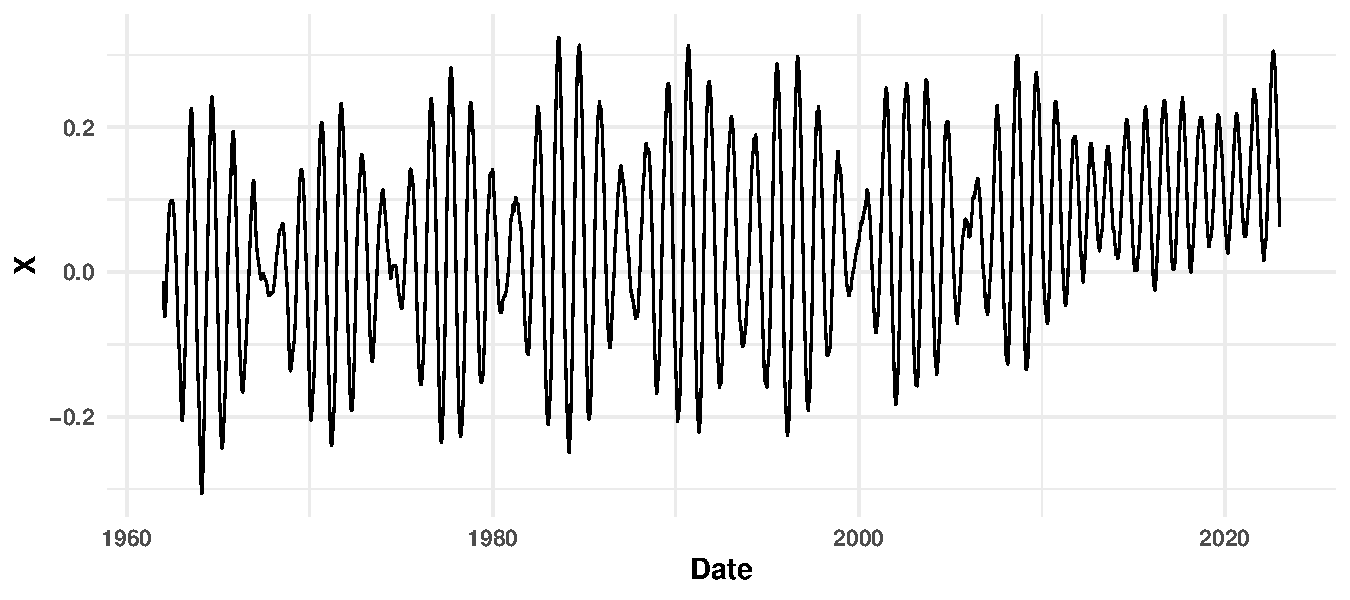
\includegraphics[width=0.51\textwidth]{Earth_x.pdf}
    };
  \end{tikzpicture}

  \begin{tikzpicture}[remember picture, overlay]
    \node[left=3.3cm, below=2.3cm] at (current page.north east)
    {
      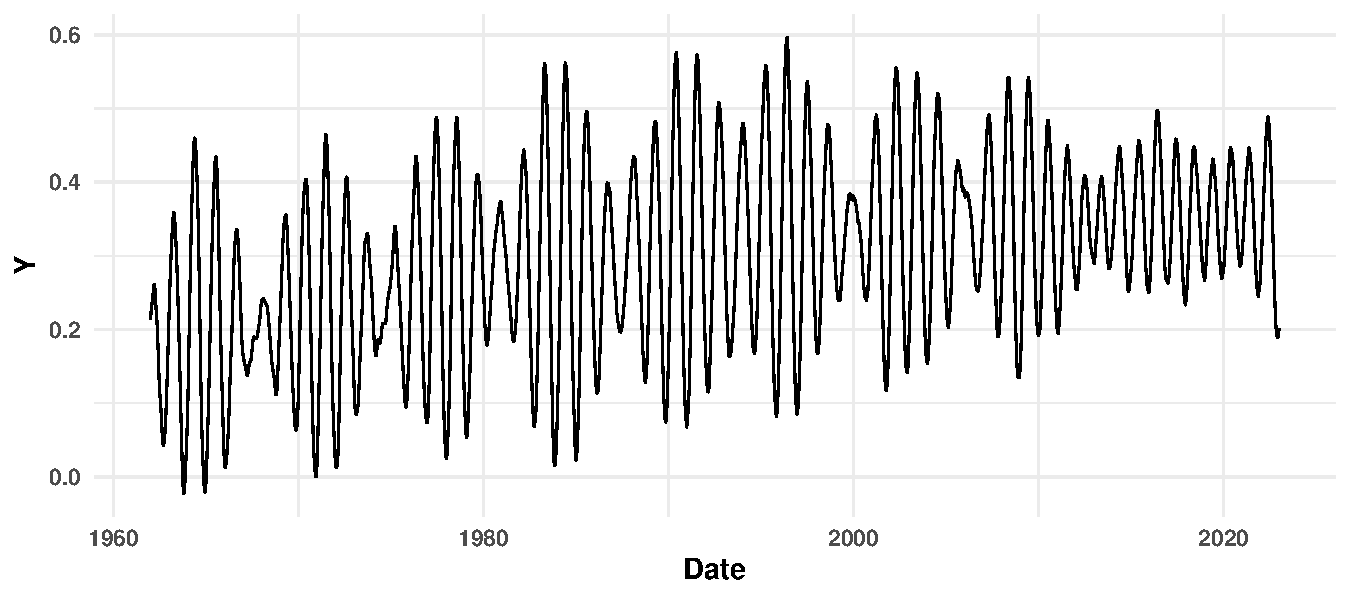
\includegraphics[width=0.51\textwidth]{Earth_y.pdf}
    };
  \end{tikzpicture}

  \begin{tikzpicture}[remember picture, overlay]
    \node[left=4.2cm, above=0.3cm] at (current page.south east)
    {
      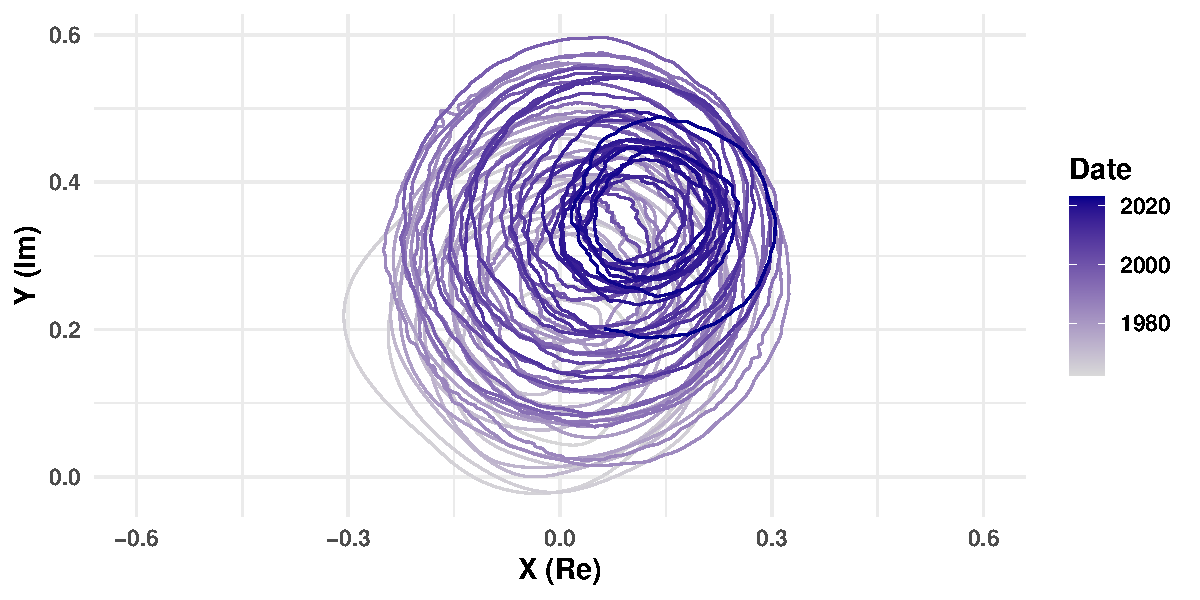
\includegraphics[width=0.62\textwidth]{Earth_complex.pdf}
    };
  \end{tikzpicture}

  \begin{columns}
    \begin{column}{0.03\textwidth}

    \end{column}
    \begin{column}{0.417\textwidth}
      As complex time series:
    \end{column}
    \begin{column}{0.58\textwidth}

    \end{column}
  \end{columns}

  \vspace{1.6cm}

\end{frame}

\begin{frame}{Decomposition and Estimation Example}
  Decomposition of time series:
  \begin{itemize}
    \item Low-frequency component + high-frequency component
    \item \bluetext{Signal + noise}
    \item Trend + Seasonality + Noise
  \end{itemize}

  \bigskip

  \begin{columns}
    \begin{column}{0.5\textwidth}
      Extracted signal:
      \begin{figure}[!ht]
        \center
        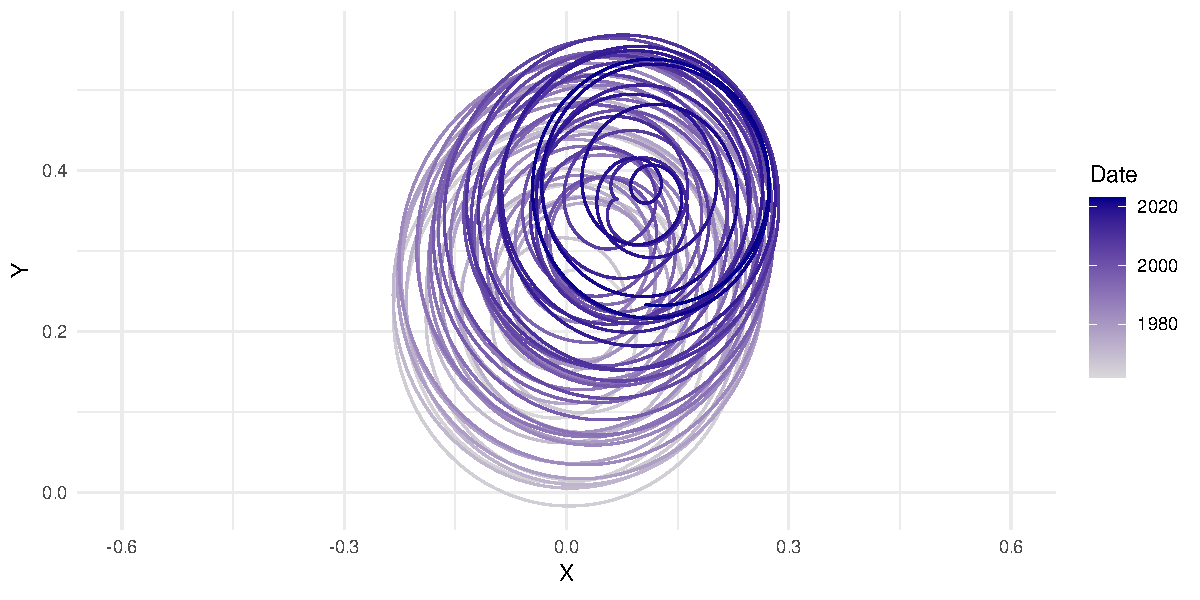
\includegraphics[width=\textwidth]{Earth_complex_signal.pdf}\\
      \end{figure}
    \end{column}
    \begin{column}{0.5\textwidth}
      Signal parameters estimates:
      \begin{table}
        \centering
        \begin{tabular}{c|c}
          Period (Days) & Change rate \\ \hline
          $365.41$ & $-5.5 \cdot 10^{-6}$ \\ \hline
          $433.10$ & $-2.2 \cdot 10^{-5}$ \\ \hline
          $\to \infty$ & $\phantom{-}2.7 \cdot 10^{-5}$
        \end{tabular}
      \end{table}
      \vspace*{0.6cm}
    \end{column}
  \end{columns}
\end{frame}

% \begin{frame}{SSA Decomposition Example}
%   Decomposition of time series:
%   \begin{itemize}
%     \item Low-frequency component + high-frequency component
%     \item \bluetext{Signal + noise}
%     \item Trend + Seasonality + Noise
%   \end{itemize}

%   \begin{figure}[!ht]
%     \center
%     \includegraphics[draft, width=0.8\textwidth,
%     height=0.5\textheight]{example-image}\\
%     *Some data*: demonstration of series decomposition with SSA
%   \end{figure}
% \end{frame}

% \begin{frame}{ESPRIT Frequency Estimation Example}
%   ESPRIT --- SSA-related method for parameters estimation.\\
%   Data: Coordinates of Earth pole motion
%   \vspace{2.7cm}

%   \begin{tikzpicture}[remember picture, overlay]
%     \node[right=3.2cm, below=2.6cm] at (current page.north west)
%     {
%       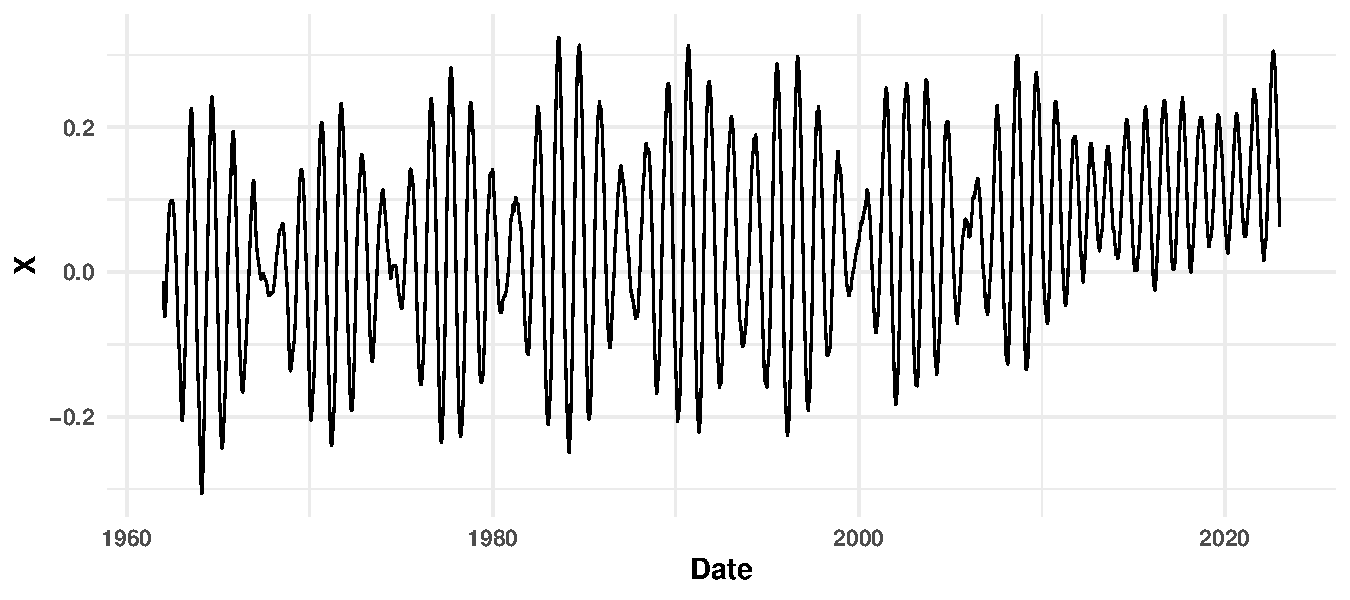
\includegraphics[width=0.48\textwidth]{Earth_x.pdf}
%     };
%   \end{tikzpicture}

%   \begin{tikzpicture}[remember picture, overlay]
%     \node[right=3.2cm, above=1.5cm] at (current page.south west)
%     {
%       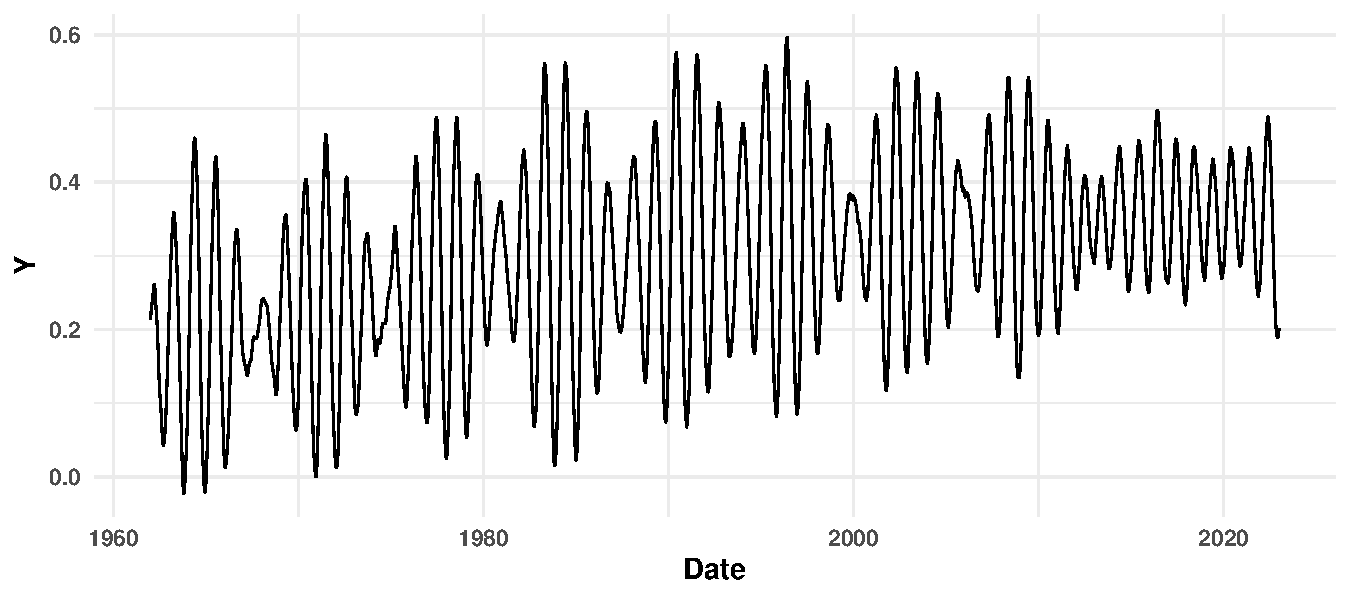
\includegraphics[width=0.48\textwidth]{Earth_y.pdf}
%     };
%   \end{tikzpicture}

%   \begin{tikzpicture}[remember picture, overlay]
%     \node[left=3.4cm, above=-1.2cm] at (current page.east)
%     {
%       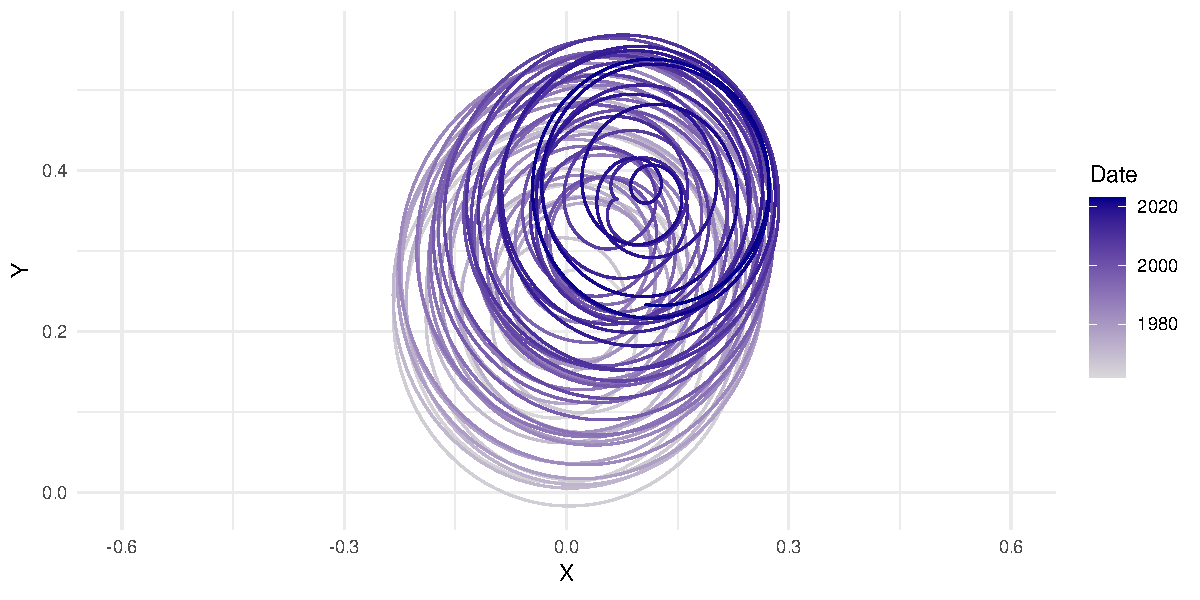
\includegraphics[width=0.52\textwidth]{Earth_complex_signal.pdf}
%     };
%   \end{tikzpicture}

%   \begin{columns}
%     \begin{column}{0.5\textwidth}

%     \end{column}
%     \begin{column}{0.49\textwidth}
%       Estimates:
%       \begin{table}
%         \centering
%         \begin{tabular}{c|c}
%           Period (Days) & Damping rate \\ \hline
%           $365.41$ & $-5.5 \cdot 10^{-6}$ \\ \hline
%           $433.10$ & $-2.2 \cdot 10^{-5}$ \\ \hline
%           $\to \infty$ & $\phantom{-}2.7 \cdot 10^{-5}$
%         \end{tabular}
%       \end{table}
%     \end{column}
%     \begin{column}{0.01\textwidth}

%     \end{column}
%   \end{columns}

% \end{frame}

% \begin{frame}{Complex Time Series}
%   Common origins of complex-valued time series:
%   \begin{itemize}
%     \item Can be constructed from two related features
%     \item Arise as a result of applying the Fourier transform to real data
%   \end{itemize}
% \end{frame}

\begin{frame}{SSA Algorithm: Embedding}
  \textbf{Input:} time series $\tX = (x_1,\, x_2,\, \ldots, x_N)$,
  window length $L$, signal rank $r$.
  \vspace{0.4cm}\\
  \begin{enumerate}
    \item \textbf{Embedding}.
      Constructing the $L$-\emph{Trajectory} Hankel matrix $\bfX\in
      \bbC^{L \times K}$ from the series $\tX$, where $K = N - L + 1$:\\
      \[
        \bfX = \calT^{(L)}(\tX) =
        \begin{pmatrix}
          x_1                     & \tikzmarknode{A12}{x_2} &
          \tikzmarknode{A13}{x_3} & \ldots & x_K     \\
          \tikzmarknode{A21}{x_2} & x_3                     & x_4
          & \ldots & x_{K+1} \\
          \tikzmarknode{A31}{x_3} & x_4                     & x_5
          & \ldots & x_{K+2} \\
          \vdots                  & \vdots                  & \vdots
          & \ddots & \vdots  \\
          x_L                     & x_{L+1}                 & x_{L+2}
          & \ldots & x_N
        \end{pmatrix}
      \]
      \begin{tikzpicture}[remember picture,overlay]
        \draw[red] let \p1=($(A12)-(A21)$),\n1={atan2(\y1,\x1)} in
        node[rotate fit=\n1,fit=(A12) (A21),draw,rounded
        corners,inner sep=2pt]{};
        \draw[blue] let \p1=($(A13)-(A31)$),\n1={atan2(\y1,\x1)+2} in
        node[rotate fit=\n1,fit=(A13) (A31),draw,rounded
        corners,inner sep=2pt]{};
      \end{tikzpicture}
  \end{enumerate}

  \bigskip

  \bluetext{Why not embed into a higher order array (tensor)?}
\end{frame}

\begin{frame}{SSA Algorithm: Decomposition, Grouping, Reconstruction}
  \begin{enumerate}
      \setcounter{enumi}{1}
    \item \textbf{Decomposition}.
      Constructing the singular value decomposition (SVD) of the matrix $\bfX$:
      $\displaystyle \bfX = \sum_{j=1}^{\operatorname{rank}\bfX}
      \sqrt{\lambda_j} U_j V_j^{\rmH} =
      \sum_{j=1}^{\operatorname{rank}\bfX} \widehat{\bfX}_j$
      where $\rmH$ denotes Hermitian
      conjugation, $U_j$ and $V_j$ are left and right singular vectors
      of $\bfX$, $\sqrt{\lambda_j}$ --- its singular values in
      descending order.
      \vspace{0.2cm}\\
    \item \textbf{Grouping}. Grouping the terms $\widehat{\bfX}_j$
      from the decomposition related to the signal:
      $\displaystyle \bfS = \sum_{j=1}^{r}\widehat{\bfX}_j = \Pi_r \bfX$,
      where $\Pi_r$ is the projector onto the space of matrices with
      rank not greater than $r$.
      \vspace{0.2cm}
    \item \textbf{Reconstruction}. Applying projection onto the
      space of Hankel
      matrices: $\widetilde{\bfS}= \Pi_{\calH}\widehat{\bfS}$,
      and return to the series form: $\widetilde{\tS}=
      \left(\calT^{(L)}\right)^{-1}(\widetilde{\bfS})$
  \end{enumerate}
\end{frame}

\begin{frame}{SSA-Rank of a Series}
  \begin{definition}
    Series $\tX$ has rank $d < N/2$ in terms of SSA, if the rank of
    its $L$-trajectory matrix equals $d$ for any $L$ such that $d
    \leqslant \min(L,
    N - L + 1)$.\\
    If such $d$ exists, then $\tX$ is called a series of finite rank.
  \end{definition}
  \vspace{0.5cm}
  If the signal $\tS$ is a series of finite rank, then it is
  generally recommended to use $\operatorname{rank}(\tS)$ as
  parameter $r$ in the SSA method
  \vspace{0.4cm}\\
  Series rank examples
  \begin{itemize}
    \item rank of $\tS$ with $s_n = A \exp(\alpha n)$, $\alpha
      \in\bbC$, equals 1
    \item rank of $\tS$ with $s_n = A\sin(2\pi \omega n + \varphi)$,
      $0 < \omega < 1/2$, equals 2
  \end{itemize}
\end{frame}

\begin{frame}{Signal Model}
  What we consider a signal $\tS = (s_1,\, s_2,\, \ldots, s_N)$:\smallskip
  \begin{itemize}
    \item The trajectory matrix $\bfS = \calT^{(L)}(\tS)$ is rank-deficient \\
      ($\implies$ the time series is of some finite rank:
      $\operatorname{rank}(\tS)=r$)
      \medskip
    \item Any signal $\tS$ can be represented in the form of a finite sum:
      \[
        s_n = \sum_{j} p_j(n) \exp(\alpha_j n + \mathrm{i}2\pi
        \omega_j n),
      \]
      where $p_j(n)$ is a polynomial in $n$
      \medskip
    \item Real case:
      \[
        s_n = \sum_{j} p_j(n) \exp(\alpha_j n)\sin(2\pi
        \omega_j n + \varphi_j),
      \]
  \end{itemize}
  \bigskip
  ESPRIT method estimates factors $\alpha_j$ and
  frequencies $\omega_j$
\end{frame}

\begin{frame}{ESPRIT Algorithm: General Idea}
  Consider a signal $\tS$ with elements $s_n$:
  \[
    s_n = \sum_{j=1}^{2} \exp(\alpha_j n + \mathrm{i}(2\pi
    \omega_j n + \varphi_j)) = A_1 z_1^n + A_2 z_2^n
  \]
  where $A_j = \exp(\mathrm{i} \varphi_j)$, $z_j = \exp(\alpha_j +
  \mathrm{i}2\pi\omega_j)$ \vspace{0.4cm}\\
  Signal subspace basis is given by
  \[
    \bfM =
    \begin{pmatrix}
      z_1 & z_2 \\
      z_1^2 & z_2^2\\
      \vdots & \vdots \\
      z_1^L & z_2^L
    \end{pmatrix} \Rightarrow \overline{\bfM} = \underline{\bfM}
    \begin{pmatrix}
      z_1 & \\ & z_2
    \end{pmatrix}\Rightarrow  \underline{\bfM}^{-}\overline{\bfM} =
    \begin{pmatrix}
      z_1 & \\ & z_2
    \end{pmatrix}
  \]
  where $\overline{\bfM}$ denotes $\bfM$ without the first row,
  $\underline{\bfM}$ --- without the last\\
  $\underline{\bfM}^{-}$ denotes the pseudoinverse of $\underline{\bfM}$
\end{frame}

\begin{frame}{ESPRIT Algorithm}
  \textbf{Input}: same as in SSA: $\tX$, $L$, $r$
  \begin{enumerate}
    \item \textbf{Embedding}. $\bfX = \calT^{(L)}(\tX)$
    \item \textbf{Decomposition}.
      $\displaystyle\bfX = \sum_{j=1}^{\operatorname{rank}\bfX}
      \sqrt{\lambda_j} U_j V_j^{\rmH}$,
      $\bfU_r = \left[U_1: U_2: \ldots: U_r\right]$
    \item \textbf{Estimation}. Finding eigenvalues $z_j$ of matrix
      $\underline{\bfU}_r^{-}\overline{\bfU}_r$ \\ \smallskip
      From $z_j = \exp(\alpha_j + \mathrm{i}2\pi\omega_j)$
      parameters $\alpha_j$ and $\omega_j$ can be found
  \end{enumerate}
\end{frame}

\begin{frame}{Multi-Channel Time Series, MSSA}
  $\tX = \left(\tX^{(1)},\, \tX^{(2)}, \, \ldots,\,
  \tX^{(P)}\right), \qquad\tX^{(p)} = \left(x_1^{(p)}, \, x_2^{(p)},\,
  \ldots,\,  x_N^{(p)}\right)$ -- channels
  \vspace{0.4cm}

  The only change in the algorithms --- Embedding step:
  \[
    \bfX = \calT_{\textrm{MSSA}}^{(L)}(\tX) = \left[\bfX^{(1)} :
    \bfX^{(2)}: \ldots : \bfX^{(P)}\right],
  \]
  \[
    \bfX^{(p)} = \calT^{(L)}(\tX^{(p)})
  \]
  \vspace{0.4cm}

  When to choose MSSA over SSA for each channel:
  \begin{itemize}
    \item All channels have ``similar'' structure
    \item ``Supporting'' channels with lower noise level
  \end{itemize}
\end{frame}

\begin{frame}{MSSA Trajectory Matrix}
  $\tX = \left(\tX^{(1)},\, \tX^{(2)}, \, \ldots,\,
  \tX^{(P)}\right), \qquad\tX^{(p)} = \left(x_1^{(p)}, \, x_2^{(p)},\,
  \ldots,\,  x_N^{(p)}\right)$
  \bigskip

  \begin{gather*}
    \bfX = \calT^{(L)}_{\mathrm{MSSA}}(\tX) =\\
    \left(
      \begin{NiceArray}{ccccc|ccccc|c}
        x_1^{(1)} & \tikzmarknode{A12}{x_2^{(1)}} &
        \tikzmarknode{A13}{x_3^{(1)}} &
        \ldots & x_K^{(1)} &
        x_1^{({\color{red}2})} & \tikzmarknode{A12}{x_2^{({\color{red}2})}} &
        \tikzmarknode{A13}{x_3^{({\color{red}2})}} &
        \ldots & x_K^{({\color{red}2})}  & \ldots \\
        \tikzmarknode{A21}{x_2^{(1)}} & x_3^{(1)} & x_4^{(1)} &
        \ldots & x_{K+1}^{(1)} & \tikzmarknode{A21}{x_2^{({\color{red}2})}} &
        x_3^{({\color{red}2})} & x_4^{({\color{red}2})} &
        \ldots & x_{K+1}^{({\color{red}2})} & \ldots \\
        \tikzmarknode{A31}{x_3^{(1)}} & x_4^{(1)} & x_5^{(1)} &
        \ldots & x_{K+2}^{(1)} & \tikzmarknode{A31}{x_3^{({\color{red}2})}} &
        x_4^{({\color{red}2})} & x_5^{({\color{red}2})} &
        \ldots & x_{K+2}^{({\color{red}2})} & \ldots \\
        \vdots                  & \vdots & \vdots & \ddots & \vdots &
        \vdots                  & \vdots & \vdots & \ddots & \vdots & \ldots  \\
        x_L^{(1)}                     & x_{L+1}^{(1)} & x_{L+2}^{(1)}
        & \ldots & x_N^{(1)} & x_L^{({\color{red}2})}                     &
        x_{L+1}^{({\color{red}2})} & x_{L+2}^{({\color{red}2})}
        & \ldots & x_N^{({\color{red}2})} & \ldots \\
        \CodeAfter
        \UnderBrace[shorten,yshift=1.5mm]{last-1}{last-5}{\bfX^{(1)}}
        \UnderBrace[shorten,yshift=1.5mm]{last-6}{last-10}{\bfX^{(2)}}
      \end{NiceArray}
    \right)
  \end{gather*}
  % \begin{tikzpicture}[remember picture,overlay]
  %   \draw[red] let \p1=($(A12)-(A21)$),\n1={atan2(\y1,\x1)} in
  %   node[rotate fit=\n1,fit=(A12) (A21),draw,rounded
  %   corners,inner sep=2pt]{};
  %   \draw[blue] let \p1=($(A13)-(A31)$),\n1={atan2(\y1,\x1)+2} in
  %   node[rotate fit=\n1,fit=(A13) (A31),draw,rounded
  %   corners,inner sep=2pt]{};
  % \end{tikzpicture}
\end{frame}

\begin{frame}[plain, c, noframenumbering]
  \vfill{}
  \begin{center}
    \huge But why limit yourself to matrices?\\
    Matrix is just a 2D tensor
  \end{center}
  \vfill{}
\end{frame}

\begin{frame}{Introducing Tensors to the Algorithm}
  \begin{table}
    \hspace*{-0.9cm}
    \begin{tabular}{rlllll}
      \bluetext{Basic SSA:} & Time series $\tX$ & $\mapsto$ & Matrix
      $\mathbf{X}$ & $\mapsto$ & $\operatorname{SVD}(\mathbf{X})$ \\
      \bluetext{Tensor SSA:} & Time series $\tX$ & $\mapsto$ & Tensor
      $\calX $ & $\mapsto$ & \hspace*{-0.18cm}
      $\underbrace{\operatorname{TD}}_{\mathclap{\text{~~~Some Tensor
      Decomposition}}}(\calX)$
    \end{tabular}
  \end{table}
  \vspace{0.4cm}

  Tensor SVD Generalizations:
  \begin{itemize}
    \item \bluetext{Higher-Order SVD (HOSVD)}
    \item Canonical Polyadic Decomposition (CPD)
    \item T-SVD
    \item $(L_r, L_r, 1)$-Decomposition
  \end{itemize}
\end{frame}

\begin{frame}{Reminder: Trajectory Matrix}
  \begin{itemize}
    \item Single-Channel:
  \end{itemize}
  \begin{gather*}
    \calT^{(L)}(\tX) =
    \begin{pmatrix}
      x_1 & x_2 & x_3 & \ldots & x_K     \\
      x_2 & x_3 & x_4 & \ldots & x_{K+1} \\
      x_3 & x_4 & x_5 & \ldots & x_{K+2} \\
      \vdots & \vdots & \vdots & \ddots & \vdots  \\
      x_L & x_{L+1} & x_{L+2} & \ldots & x_N \\
    \end{pmatrix}
  \end{gather*}
  \begin{itemize}
    \item Multi-Channel:
  \end{itemize}
  \begin{gather*}
    \calT_{\mathrm{MSSA}}^{(L)}(\tX) =
    \left(
      \begin{NiceArray}{cccc|cccc|c}
        x_1^{(1)} & x_2^{(1)} & \ldots & x_K^{(1)} &
        x_1^{({\color{red}2})} & x_2^{({\color{red}2})} & \ldots
        & x_K^{({\color{red}2})}  & \ldots \\
        x_2^{(1)} & x_3^{(1)} & \ldots & x_{K+1}^{(1)} &
        x_2^{({\color{red}2})} &
        x_3^{({\color{red}2})} & \ldots &
        x_{K+1}^{({\color{red}2})} & \ldots \\
        \vdots & \vdots & \ddots & \vdots &
        \vdots & \vdots & \ddots &
        \vdots & \ldots  \\
        x_L^{(1)} & x_{L+1}^{(1)} & \ldots & x_N^{(1)} &
        x_L^{({\color{red}2})} & x_{L+1}^{({\color{red}2})} &
        \ldots & x_N^{({\color{red}2})} & \ldots \\
      \end{NiceArray}
    \right)
  \end{gather*}
\end{frame}

\begin{frame}{Mapping Single-Channel Time Series to a Tensor}
  $\tX = (x_1,\, x_2,\, \ldots,\, x_N)$\\ \medskip
  $\tX \mapsto \calT_{\mathrm{T-SSA}}^{(I, L)}(\tX) = \calX \in
  \bbC^{I\times L \times K}$, $K = N - I - L + 2$

  \begin{figure}[!ht]
    \centering
    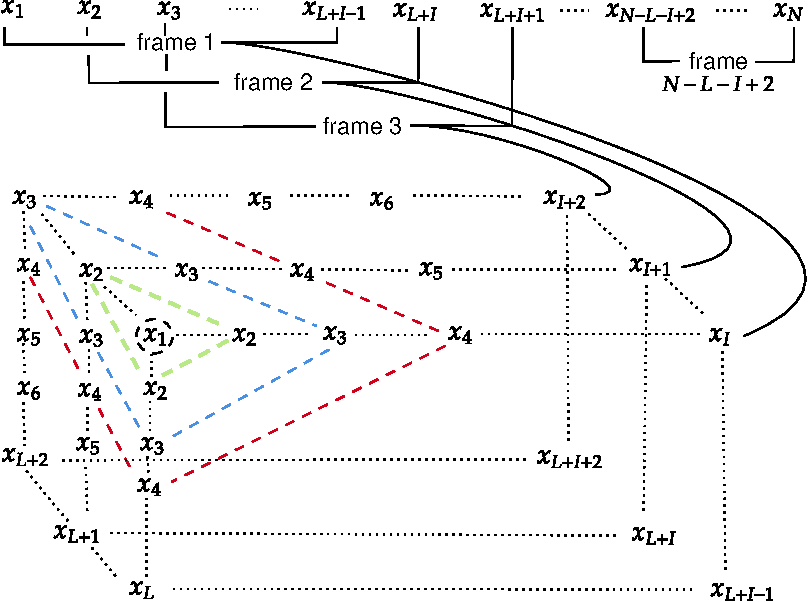
\includegraphics[width=0.7\textwidth]{tens-injection-wide.pdf}
  \end{figure}
\end{frame}

\begin{frame}{Mapping Multi-Channel Time Series to a Tensor}
  $\tX = \left(\tX^{(1)},\, \tX^{(2)},\, \ldots,\,
  \tX^{(P)}\right)$, $\tX^{(p)} = (x_1^{(p)},\, x_2^{(p)},\,
  \ldots,\, x_N^{(p)})$\\ \medskip
  $\tX \mapsto \calT_{\mathrm{T-MSSA}}^{(L)}(\tX)
  = \calX \in \bbC^{P\times L \times K}$, $K = N - L + 1$

  \bigskip

  \begin{figure}[!ht]
    \centering
    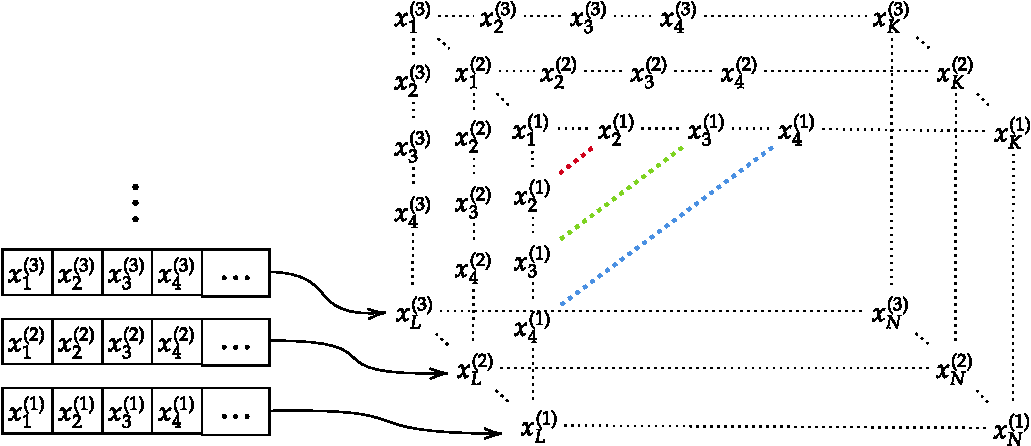
\includegraphics[width=0.8\textwidth]{mssa_injection_new.pdf}
  \end{figure}
\end{frame}

\begin{frame}{Some Tensor Decompositions}
  Unlike in matrix case, there exist several definitions of tensor ranks and
  SVD generalizations based on them.

  \begin{definition}[Tensor rank]
    Tensor $\calA$ has rank 1, if there exist vectors $B$, $C$ and $D$ such that
    $\calA=B \circ C \circ D$, where $\circ$ denotes an outer
    product.\\ \medskip

    Tensor $\calA$ has rank $R$, if it can be represented as a sum of
    $R$ rank-1 tensors: $\calA = \sum_{i=1}^{R} \calB_i$,
    $\operatorname{rank}(\calB_i)=1$, and such $R$ is minimal.
  \end{definition}

  \medskip

  The representation of a tensor as a sum of $R$ rank-1 tensors is called
  \bluetext{Canonical Polyadic Decomposition (CPD)}.

  \smallskip

  \begin{itemize}
    \item Considered for signal extraction in [Kouchaki, Sanei (2013)]
    \item Does not provide any form of orthogonality of components
    \item Requires to know the tensor rank in advance
    \item No connection between signal SSA-rank and the rank of a
      trajectory tensor
  \end{itemize}
  %   \medskip
  % \item \bluetext{T-SVD}: $\calA = \calU * \calS * \calV^\rmH$,
  %   where $\calD = \calB * \calC \Leftrightarrow d_{ilk} = \sum_{j}
  %   b_{ijk} c_{jlk}$, subindex $\rmH$ denotes complex conjugation of
  %   all frontal slices, $\calU = \calU^{\rmH}$, $\calV = \calV^{\rmH}$,
  %   all frontal slices of $\calS$ are diagonal matrices (tubal form)
  %   \begin{itemize}
  %     \item Considered for signal extraction and decomposition in
  %       [Trung~et~al.~(2024)]
  %     \item Provides some orthogonality
  %     \item Numerical experiments show less precision than
  %       matrix-based methods
  %   \end{itemize}
\end{frame}

\begin{frame}{Some tensor decompositions}
  \begin{definition}
    \bluetext{$n$-mode vectors} of a tensor $\calA$ are vectors
    obtained from $\calA$ by varying the index of the
    $n$-th direction and keeping the other indices fixed (analog of
    rows and columns of a matrix).\\ \medskip

    \bluetext{$n$-rank} of a tensor $\calA$, denoted by $R_n =
    \operatorname{rank}_n(\calA)$, is the dimension of the linear
    space spanned by the $n$-mode vectors.
  \end{definition}

  \medskip

  \bluetext{HOSVD}: $\calA = \sum_{i=1}^{R_1}\,
  \sum_{l=1}^{R_2}\, \sum_{k=1}^{R_3}\, z_{ilk} U_i^{(1)} \circ
  U_l^{(2)} \circ U_k^{(3)}$
  \begin{itemize}
    \item Considered for signal parameter estimation in [Papy et
      al. (2005)], [Papy et al. (2009)]
    \item Provides orthogonality of components
    \item Does not require any prior knowledge about tensor $n$-ranks
    \item There is a proven connection between number of components
      and signal SSA-rank
  \end{itemize}
\end{frame}

\begin{frame}{Higher-Order SVD. Higher-Order Orthogonal Iterations}
  \vspace*{-0.7cm}
  \begin{align*}
    \operatorname{SVD}(\bfX) &= \sum_{j=1}^{\operatorname{rank}(\bfX)}
    \sqrt{\lambda_j} U_j V_j^{\rmH}\\
    \operatorname{HOSVD}(\calX) &=
    \sum_{i=1}^{\operatorname{rank}_{\color{red}1}(\calX)}\,
    \sum_{l=1}^{\operatorname{rank}_{\color{red}2}(\calX)}\,
    \sum_{k=1}^{\operatorname{rank}_{\color{red}3}(\calX)}\,
    z_{ilk} U_i^{(1)} \circ U_l^{(2)} \circ U_k^{(3)}
  \end{align*}

  \begin{itemize}
    \item $\displaystyle \widetilde{\bfX} =
      \sum_{j=1}^{R}\ldots \Rightarrow
      \left\| \bfX - \widetilde{\bfX} \right\|_{F} =
      \min_{\operatorname{rank}(\widehat{\bfX}) \leqslant R}\left\|
      \bfX - \widehat{\bfX}\right\|_F$
    \item $\displaystyle \widetilde{\calX}=
      \sum_{i=1}^{R_1}\,
      \sum_{l=1}^{R_2}\,
      \sum_{k=1}^{R_3}\,
      \ldots \Rightarrow
      \left\| \calX - \widetilde{\calX} \right\|_{F} \geqslant
      \min_{\operatorname{rank}_{m}(\widehat{\calX}) \leqslant R_m}\left\|
      \calX - \widehat{\calX}\right\|_F$
  \end{itemize}
  \vspace{0.6cm}

  \bluetext{Truncation of SVD is optimal, but truncation of HOSVD is
  not}\vspace{0.1cm}

  Iterative algorithm for finding optimal approximation -- \bluetext{HOOI}
\end{frame}

\begin{frame}{T-SSA, T-MSSA and T-ESPRIT with HOSVD}
  \textbf{Input:} time series $\tX$,
  window length: $(I, L)$ for single-channel or $L$ for multi-channel,
  signal ranks $(r_1,\, r_2,\, r_3)$, $d$ --- estimation dimension
  for HO-ESPRIT.
  \vspace{0.4cm}\\
  \begin{enumerate}
    \item \textbf{Embedding}.
      \begin{tabular}{r|l}
        Single-channel & $\tX \mapsto\calT_{\mathrm{T-SSA}}^{(I,
        L)}(\tX) = \calX$ \\ \hline
        Multi-channel &
        $\tX \mapsto \calT_{\mathrm{T-MSSA}}^{(L)}(\tX) = \calX$
      \end{tabular}
      \vspace{0.2cm}

    \item \textbf{Decomposition \& Approximation}. Using $(r_1,\,
      r_2,\, r_3)$\\\smallskip
      $\calX \mapsto
      \operatorname{Trunc}(\operatorname{HOSVD}(\calX)) =
      \widetilde{\calS}$ or
      $\calX \mapsto \operatorname{HOOI}(\calX) = \widetilde{\calS}$
      \vspace{0.2cm}

    \item \textbf{Reconstruction or Estimation}. \\
      \begin{itemize}
        \item \textbf{Reconstruction}.
          $\tS = \calT^{-1}
          \left(\Pi_{\calH_{\mathrm{T}}} (\widetilde{\calS})\right)$,
          $\Pi_{\calH_{\mathrm{T}}}$ --- projector onto the space of
          Hankel tensors
        \item \textbf{Estimation}. Finding eigenvalues $z_j$ of
          matrix $\underline{\bfU}^{-}\overline{\bfU}$, where
          $\bfU = \bfU_d = \left[U_1^{(d)}:U_2^{(d)}:\ldots
          :U_{r_d}^{(d)}\right]$.
          From $z_j = \exp(\alpha_j + \mathrm{i}2\pi\omega_j)$
          factors $\alpha_j$ and frequencies $\omega_j$ of
          the signal can be found
      \end{itemize}
  \end{enumerate}
\end{frame}

\begin{frame}{Single-Channel Series Comparison}
  \vspace*{-0.3cm}
  \[
    x_{n} = e^{ \alpha_1 n } e^{2 \pi\mathrm{i} \omega_1 n} +
    e^{ \alpha_2 n } e^{ 2 \pi  \mathrm{i}\omega_2 n} + \zeta_n
  \]
  $\zeta_n$ --- Complex white gaussian noise, $\mathrm{D}(\zeta_n) =
  0.04^2$, $\omega_1 = 0.2,\, \omega_2 = 0.22$, $\alpha_1=\alpha_2=0$
  (same results for $\alpha_1=\alpha_2 < 0$ and $\alpha_1 < \alpha_2 < 0$).

  \medskip
  \bluetext{RMSE results with respect to parameters choice:}
  \begin{itemize}
    \item Parameters estimation
  \end{itemize}
  \begin{columns}
    \begin{column}{0.65\textwidth}
      \begin{table}[ht]
        \centering
        \begin{tabular}{c|ccc}
          \hline
          & Best & Worst & Mean \\
          \hline
          \textbf{T-ESPRIT} & \textbf{\bluetext{0.0012}} &
          \textbf{\bluetext{0.0033}} &
          \textbf{\bluetext{0.0016}} \\
          \textbf{ESPRIT} & \bluetext{0.0013} & 0.0140 & 0.0031 \\
          \hline
        \end{tabular}
        % \caption{RMSE statistics across all method parameters}
      \end{table}
    \end{column}
    \begin{column}{0.35\textwidth}
      T-method is better
    \end{column}
  \end{columns}

  \begin{itemize}
    \item Signal extraction
  \end{itemize}
  \begin{columns}
    \begin{column}{0.65\textwidth}
      \begin{table}[ht]
        \centering
        \begin{tabular}{c|ccc}
          \hline
          & Best & Worst & Mean \\
          \hline
          \textbf{T-SSA} & \bluetext{0.019} &
          \textbf{\bluetext{0.024}} &
          \textbf{\bluetext{0.020}} \\
          \textbf{SSA} & \textbf{\bluetext{0.018}} & 0.031 &
          \textbf{\bluetext{0.021}} \\
          \hline
        \end{tabular}
        % \caption{RMSE statistics across all method parameters}
      \end{table}
    \end{column}
    \begin{column}{0.35\textwidth}
      T-method is worse with optimal parameter choice.
    \end{column}
  \end{columns}
  % \begin{figure}
  %   \centering
  %   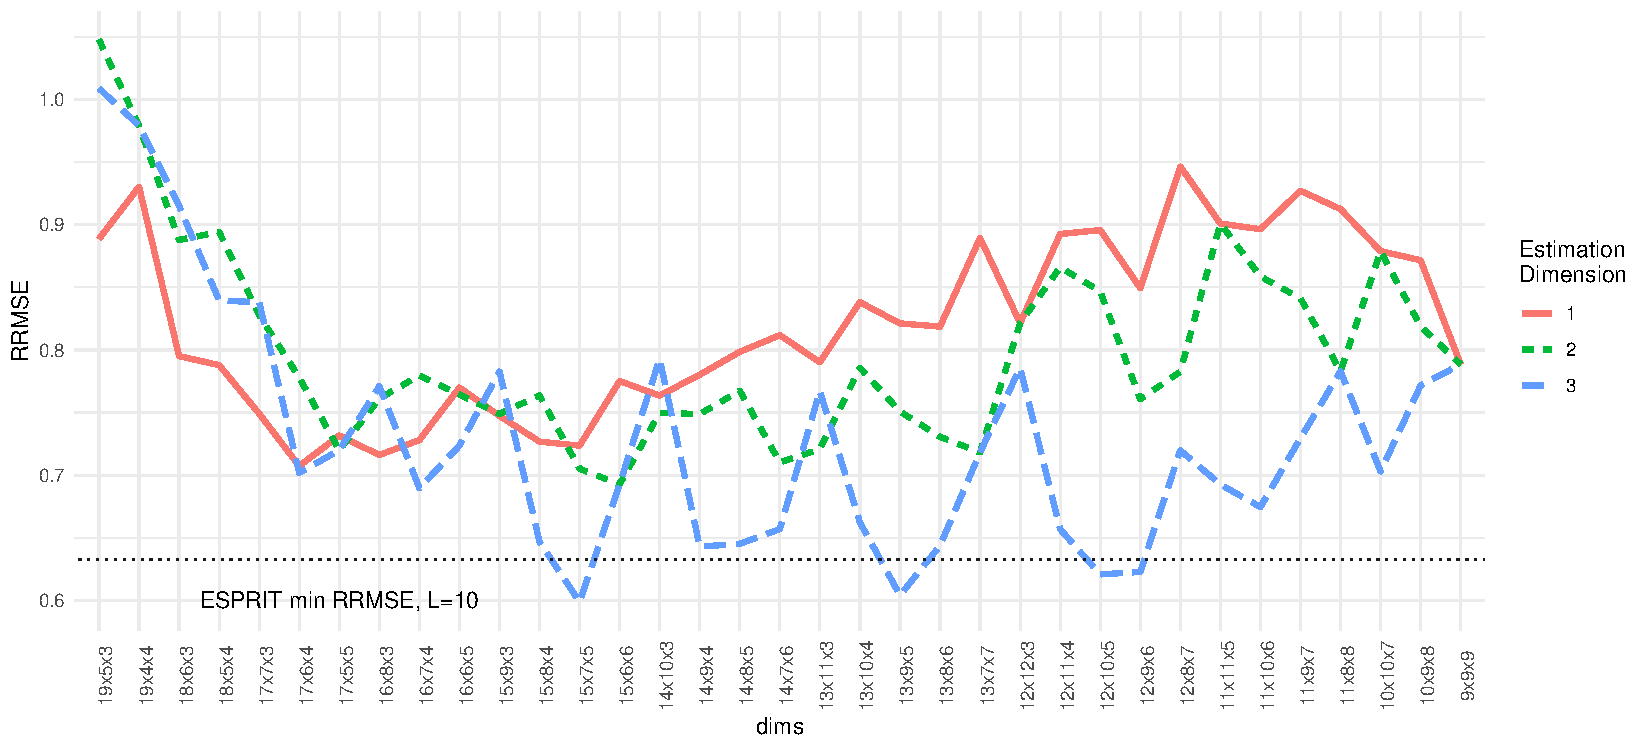
\includegraphics[width=0.89\textwidth]{img/freq1_dims_no_rates.pdf}
  %   \caption{RMSE of estimates for $\omega_1$ vs window lengths
  %   ($I\times L \times K$)}
  % \end{figure}
\end{frame}

\begin{frame}{Multi-Channel Series Comparison}
  \[
    x_{n}^{(m)} = a_1^{(m)}
    e^{2 \pi \mathrm{i} \omega_1 n} +
    a_2^{(m)}
    e^{2 \pi \mathrm{i} \omega_2 n} + \zeta_n^{(m)},
  \]
  $\zeta_n^{(m)}$ --- Complex white gaussian noise,
  $\mathrm{D}\left(\zeta_n^{(m)}\right) = 0.2^2$, $\omega_1 = 0.2,\,
  \omega_2 = 0.22$

  \medskip

  \bluetext{RMSE results with respect to parameters choice:}
  \begin{itemize}
    \item Parameters estimation
  \end{itemize}

  \begin{columns}
    \begin{column}{0.8\textwidth}
      \begin{table}[ht]
        \centering
        \begin{tabular}{c|ccc}
          \hline
          & Best & Worst & Average \\
          \hline
          \textbf{T-M-ESPRIT} & \textbf{\bluetext{5.33e-04}} &
          \textbf{\bluetext{9.99e-04}} &
          \textbf{\bluetext{6.16e-04}} \\
          \textbf{M-ESPRIT} & \bluetext{5.36e-04} & 1.80e-03
          & 7.13e-04 \\
          \hline
        \end{tabular}
      \end{table}
    \end{column}
    \begin{column}{0.2\textwidth}
      T-method is better
    \end{column}
  \end{columns}

  \begin{itemize}
    \item Signal extraction
  \end{itemize}

  \begin{columns}
    \begin{column}{0.7\textwidth}
      \begin{table}[ht]
        \centering
        \begin{tabular}{c|ccc}
          \hline
          & Best & Worst & Average \\
          \hline
          \textbf{T-MSSA} & \textbf{\bluetext{0.065}} &
          \textbf{\bluetext{0.068}} &
          \textbf{\bluetext{0.066}} \\
          \textbf{MSSA} & \bluetext{0.066} & 0.152 & 0.086 \\
          \hline
        \end{tabular}
      \end{table}
    \end{column}
    \begin{column}{0.3\textwidth}
      T-method is better
    \end{column}
  \end{columns}
\end{frame}

% \begin{frame}{Single-Channel Case Comparison, Signal Extraction}
%   \vspace*{-0.3cm}
%   \[
%     x_{n} = e^{ \alpha_1 n } e^{2 \pi\mathrm{i} \omega_1 n} +
%     e^{ \alpha_2 n } e^{ 2 \pi  \mathrm{i}\omega_2 n} + \zeta_n
%   \]
%   $\zeta_n$ --- Complex white gaussian noise,
%   $\mathrm{D}(\zeta_n) = 0.04^2$, $\omega_1 = 0.2,\,
%   \omega_2 = 0.22$, $\alpha_1=\alpha_2=0$ (same results for
%   $\alpha_1=\alpha_2 < 0$ and $\alpha_1 < \alpha_2 < 0$).

%   \begin{figure}
%     \centering
%     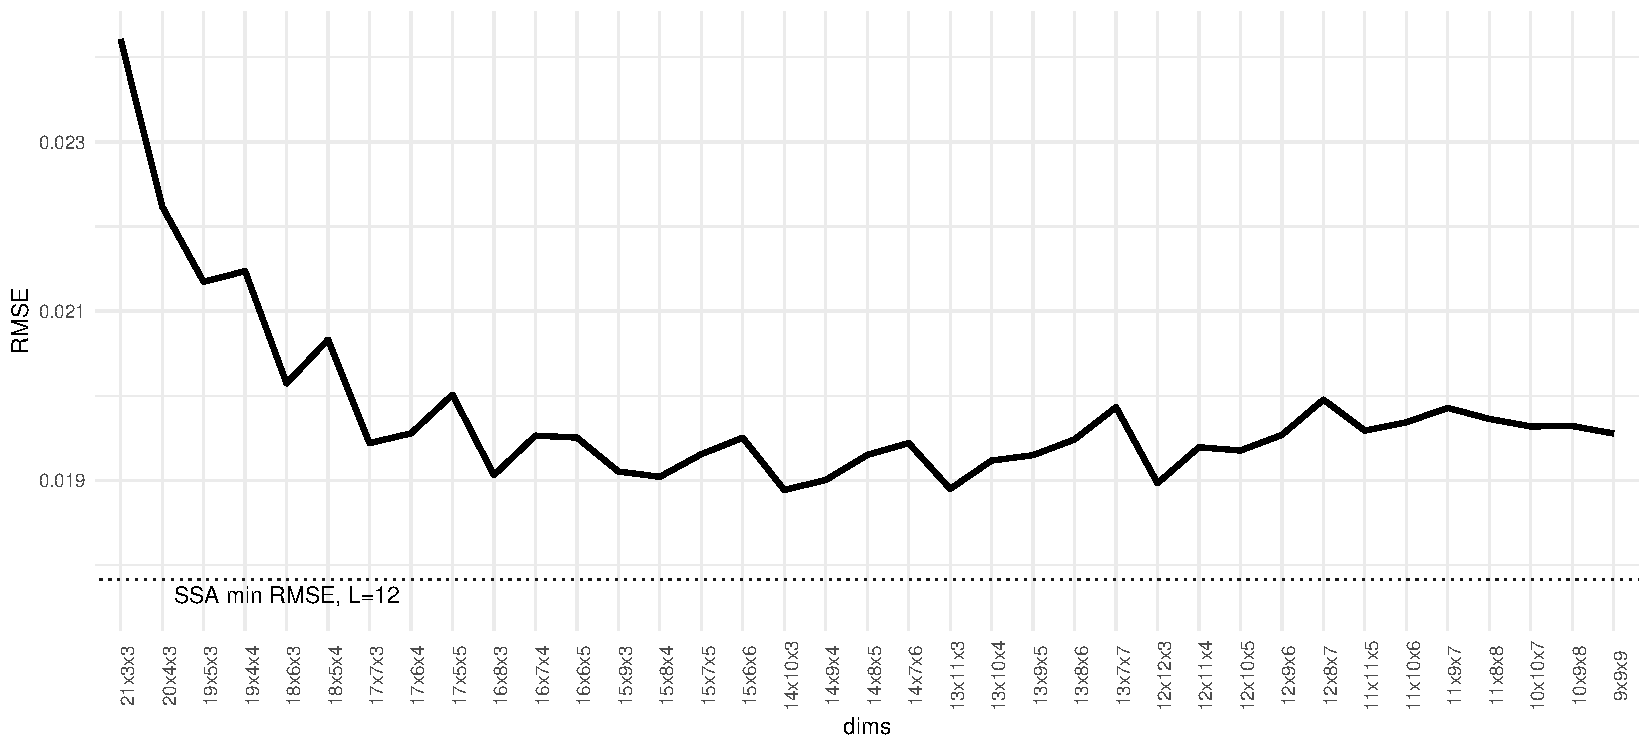
\includegraphics[width=0.89\textwidth]{img/rec_dim_rmse_no_rates.pdf}
%     \caption{RMSE of signal estimation vs window lengths
%     ($I\times L \times K$)}
%   \end{figure}
% \end{frame}

\begin{frame}{Dtack Modifications}
  Possible problem for ESPRIT: components with close frequencies can
  mix into one in the presence of noise. Solution: using Dstack mapping.
  \medskip

  Consider $\tX = (x_1,\, x_2,\, \ldots,\, x_N)$, $M = \lfloor N /
  D\rfloor$, then
  \[
    \operatorname{Dstack}_D(\tX) = \calD_D(\tX) =
    \left[
      \begin{NiceArray}{c|c|c|c}
        x_1 & x_2 & \ldots & x_{D} \\
        x_{D+1} & x_{D+2}  &\ldots &  x_{2D} \\
        x_{2D+1} & x_{2D+2} &\ldots & x_{3D} \\
        \vdots & \vdots & \ \cdots \  & \vdots \\
        x_{(M - 1)D+1} & x_{(M - 1)D+2}
        &\ldots & x_{MD} \\
        \CodeAfter
        \UnderBrace[shorten,yshift=1.5mm]{last-1}{last-1}{\tX_D^{(1)}}
        \UnderBrace[shorten,yshift=1.5mm]{last-2}{last-2}{\tX_D^{(2)}}
        \UnderBrace[shorten,yshift=1.5mm]{last-4}{last-4}{\tX_D^{(D)}}
      \end{NiceArray}
    \right]
  \]
  \vspace{0.3cm}

  \begin{table}
    \renewcommand{\arraystretch}{1.4}
    \begin{tabular}{r|l}
      Dstack-SSA & $\displaystyle\tX \mapsto \bfX=
      \calT_{\textrm{MSSA}}^{(L)} \left( \calD_D (\tX)\right)$\\\hline
      Dstack-T-SSA & $\displaystyle\tX \mapsto \calX=
      \calT_{\textrm{T-MSSA}}^{(L)} \left( \calD_D (\tX)\right)$
    \end{tabular}
  \end{table}

  Undersampling: $\displaystyle\omega \mapsto \hat\omega=
  D \omega \implies |\omega| \leqslant \frac{1}{2D}$ is required
\end{frame}

\begin{frame}{Single-Channel Series Comparison with Dstack}
  \vspace*{-0.3cm}
  \[
    x_{n} = \cos(2 \pi \omega_1 n) +
    \cos(2 \pi \omega_2 n) + \xi_n
  \]
  $\omega_1 = 0.02,\, \omega_2 = 0.0205$, $\xi_n$ --- white gaussian
  noise, $\mathrm{D}(\xi_n) = \sigma^2$

  \medskip
  \bluetext{RMSE results with respect to parameters choice:}

  \begin{itemize}
    \item Parametes estimation, $\sigma = 0.2$
  \end{itemize}

  \begin{columns}
    \begin{column}{0.9\textwidth}
      \begin{table}[ht]
        \centering
        \begin{tabular}{c|ccc}
          \hline
          & Best & Worst & Average \\
          \hline
          \textbf{ESPRIT} & \textbf{\bluetext{4.98e-05}} &
          \textbf{\bluetext{5.66e-05}} &
          \textbf{\bluetext{5.32e-05}} \\
          \textbf{Dstack-ESPRIT} & 5.30e-05 & 7.63e-05 & 6.24e-05 \\
          \textbf{T-Dstack-ESPRIT} & 5.40e-05 & 6.24e-05 & 5.86e-05 \\
          \hline
        \end{tabular}
      \end{table}
    \end{column}
    \begin{column}{0.15\textwidth}
      T-method is worse
    \end{column}
  \end{columns}

  \begin{itemize}
    \item Parametes estimation, $\sigma = 0.6$
  \end{itemize}

  \begin{columns}
    \begin{column}{0.7\textwidth}
      \begin{table}[ht]
        \centering
        \begin{tabular}{c|ccc}
          \hline
          & Best & Worst & Average \\
          \hline
          \textbf{ESPRIT} & 0.101 & 0.138 & 0.115 \\
          \textbf{Dstack-ESPRIT} & 0.009 & 0.011 & 0.010 \\
          \textbf{T-Dstack-ESPRIT} & \textbf{\bluetext{0.003}} &
          \textbf{\bluetext{0.005}} &
          \textbf{\bluetext{0.004}} \\
          \hline
        \end{tabular}
      \end{table}
    \end{column}
    \begin{column}{0.3\textwidth}
      T-method is better
    \end{column}
  \end{columns}

  % \begin{figure}[!ht]
  %   \begin{minipage}{0.48\textwidth}
  %     \centering
  %     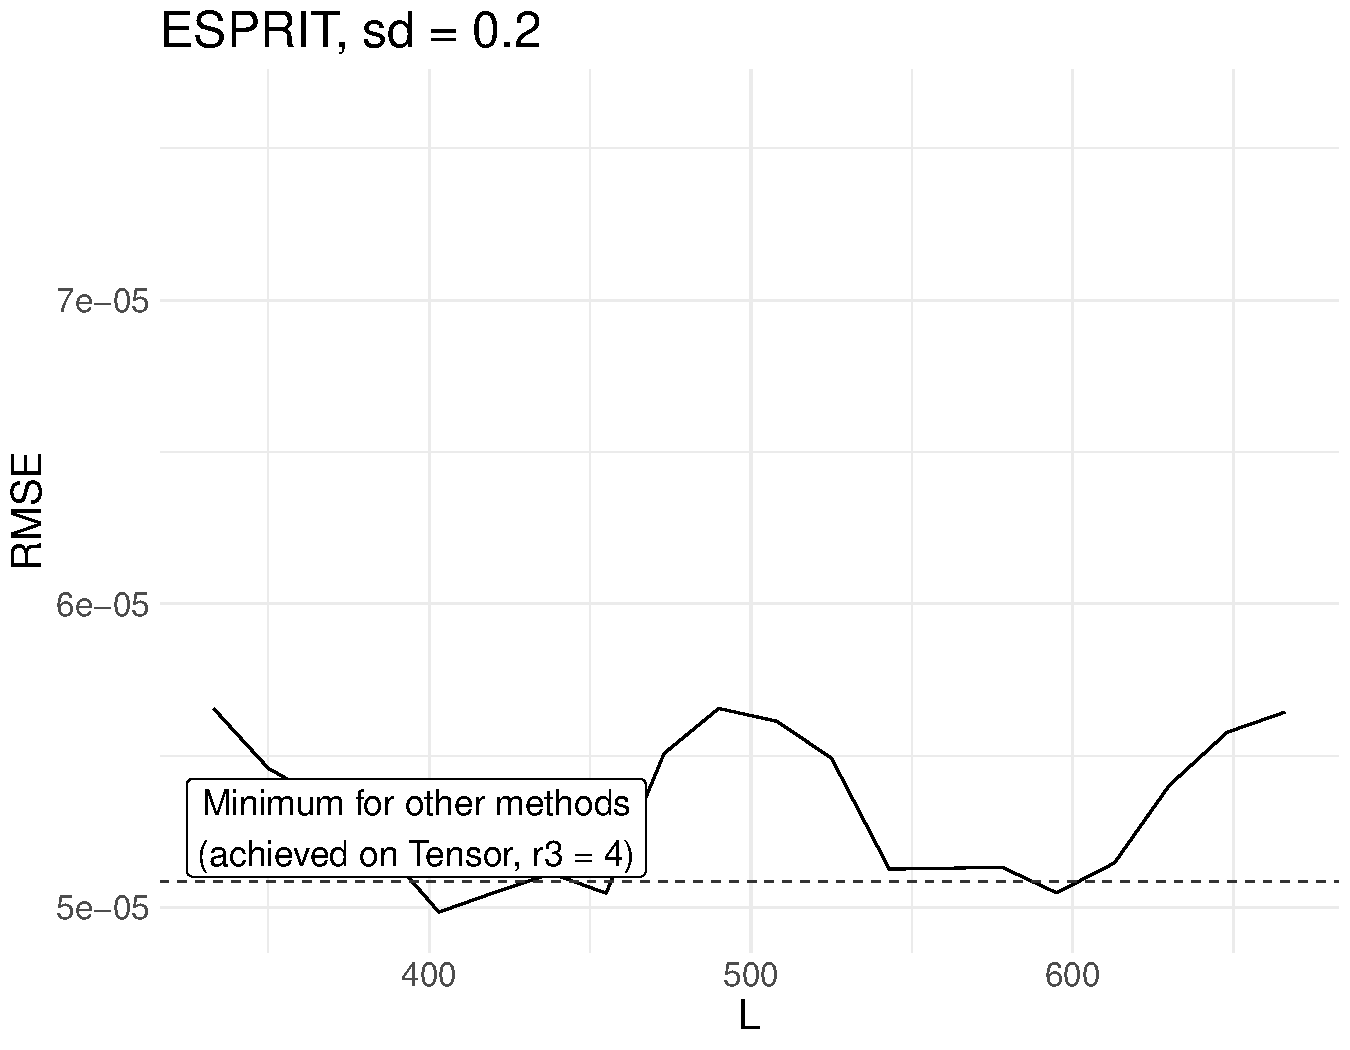
\includegraphics[width=\textwidth]{img/htlsd_byL_real_param_rmse_esprit_2.pdf}
  %   \end{minipage}
  %   \begin{minipage}{0.48\textwidth}
  %     \centering
  %     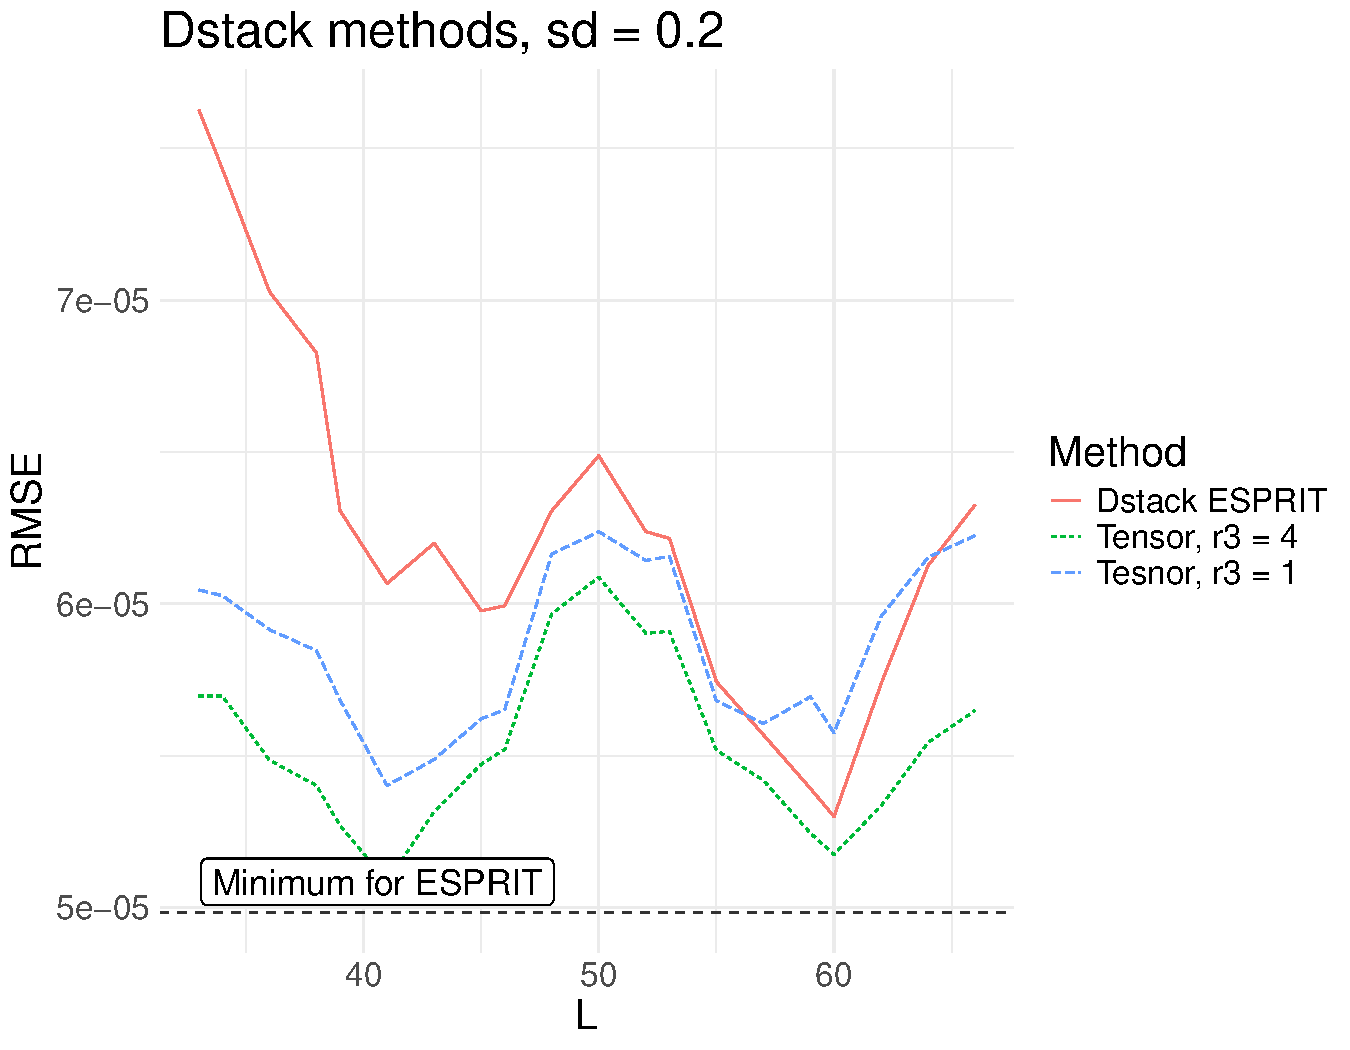
\includegraphics[width=\textwidth]{img/htlsd_byL_real_param_rmse_dstack_2.pdf}
  %   \end{minipage}
  %   \caption{RMSE of estimates for frequencies by default ESPRIT
  %   (left) and Dstack variant (right). Low noise level case.}
  % \end{figure}
\end{frame}

\begin{frame}{Single-Channel Series Comparison with Dstack}
  \vspace*{-0.3cm}
  \[
    x_{n} = \cos(2 \pi \omega_1 n) +
    \cos(2 \pi \omega_2 n) + \xi_n
  \]
  $\omega_1 = 0.02,\, \omega_2 = 0.0205$, $\xi_n$ --- white gaussian
  noise, $\mathrm{D}(\xi_n) = \sigma^2$

  \medskip
  \bluetext{RMSE results with respect to parameters choice:}

  \begin{itemize}
    \item Signal extraction, $\sigma = 0.2$
  \end{itemize}

  \begin{columns}
    \begin{column}{0.7\textwidth}
      \begin{table}[ht]
        \centering
        \begin{tabular}{c|ccc}
          \hline
          & Best & Worst & Average \\
          \hline
          \textbf{SSA} & \textbf{\bluetext{0.020}} &
          \textbf{\bluetext{0.021}} &
          \textbf{\bluetext{0.021}} \\
          \textbf{Dstack-SSA} & 0.052 & 0.066 & 0.057 \\
          \textbf{T-Dstack-SSA} & 0.050 & 0.052 & 0.051 \\
          \hline
        \end{tabular}
      \end{table}
    \end{column}
    \begin{column}{0.3\textwidth}
      T-method is worse
    \end{column}
  \end{columns}

  \begin{itemize}
    \item Signal extraction, $\sigma = 0.6$
  \end{itemize}

  \begin{columns}
    \begin{column}{0.7\textwidth}
      \begin{table}[ht]
        \centering
        \begin{tabular}{c|ccc}
          \hline
          & Best & Worst & Average \\
          \hline
          \textbf{SSA} & \textbf{\bluetext{0.086}} &
          \textbf{\bluetext{0.095}} &
          \textbf{\bluetext{0.090}} \\
          \textbf{Dstack-SSA} & 0.175 & 0.208 & 0.189 \\
          \textbf{T-Dstack-SSA} & 0.175 & 0.179 & 0.178 \\
          \hline
        \end{tabular}
      \end{table}
    \end{column}
    \begin{column}{0.3\textwidth}
      T-method is worse
    \end{column}
  \end{columns}
\end{frame}

% \begin{frame}{Single-Channel Case, Dstack Parameters Estimation}
%   \vspace*{-0.3cm}
%   \[
%     x_{n} = \cos(2 \pi \omega_1 n) +
%     \cos(2 \pi \omega_2 n) + \xi_n
%   \]
%   $\omega_1 = 0.02,\, \omega_2 = 0.0205$, $\xi_n$ --- white gaussian
%   noise, $\mathrm{D}(\xi_n) = 0.6^2$
%   \begin{figure}
%     \begin{minipage}{0.48\textwidth}
%       \centering
%       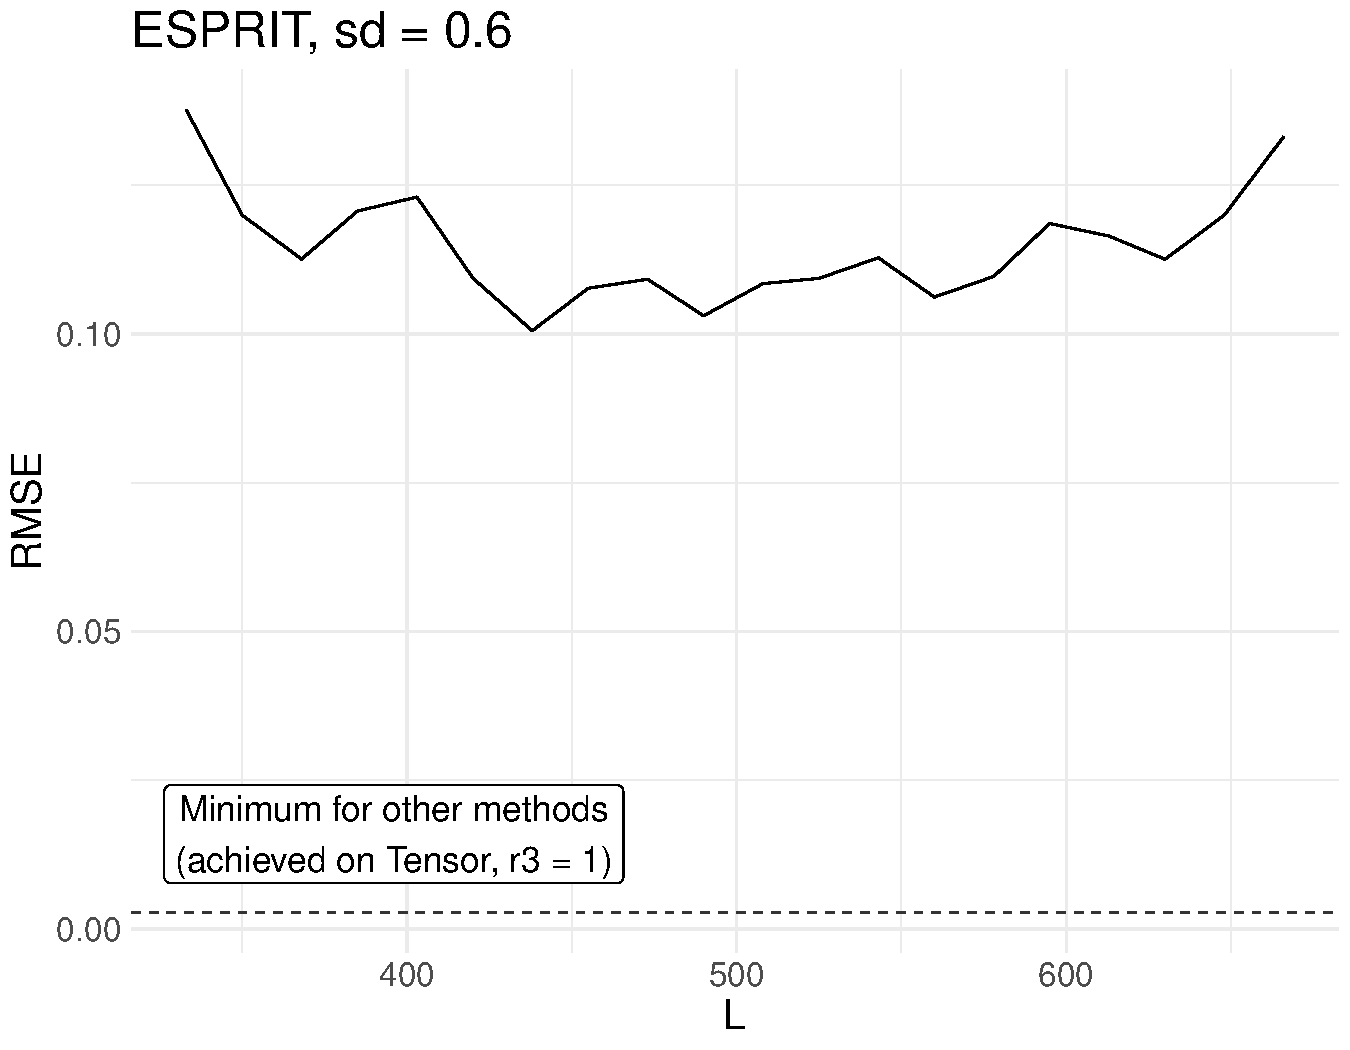
\includegraphics[width=\textwidth]{img/htlsd_byL_real_param_rmse_esprit_3.pdf}
%     \end{minipage}
%     \begin{minipage}{0.48\textwidth}
%       \centering
%       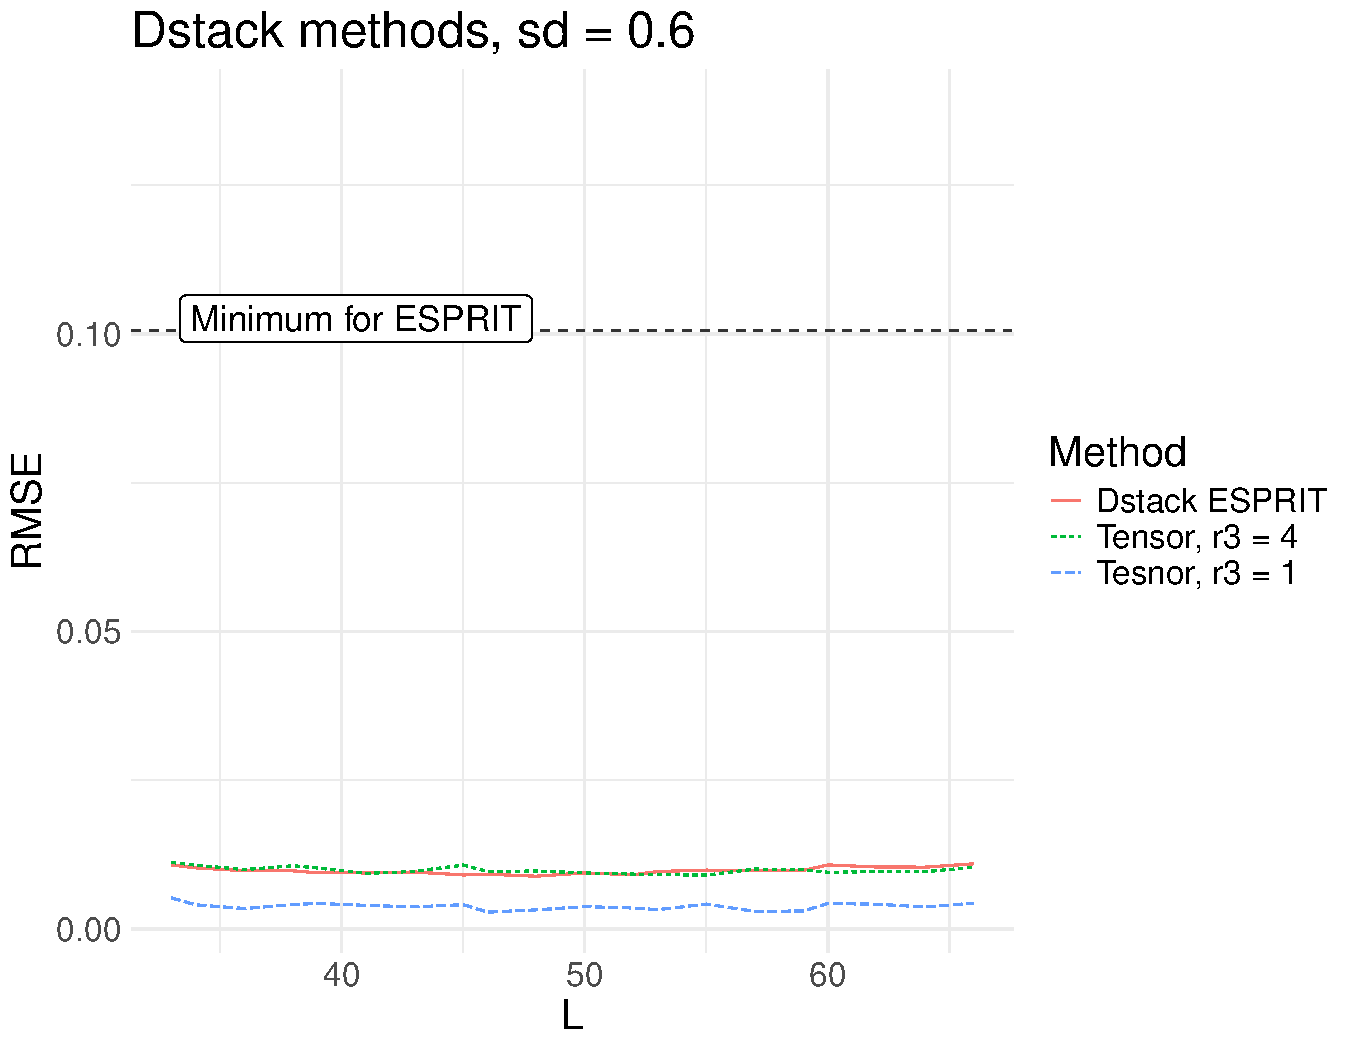
\includegraphics[width=\textwidth]{img/htlsd_byL_real_param_rmse_dstack_3.pdf}
%     \end{minipage}
%     \caption{RMSE of estimates for frequencies by default ESPRIT
%     (left) and Dstack variant (right). High noise level case.}
%   \end{figure}
% \end{frame}

% \begin{frame}{ Single-Channel Case, Dstack Signal Extraction}
%   \vspace*{-0.3cm}
%   \[
%     x_{n} = \cos(2 \pi \omega_1 n) +
%     \cos(2 \pi \omega_2 n) + \xi_n
%   \]
%   $\omega_1 = 0.02,\, \omega_2 = 0.0205$, $\xi_n$ --- white gaussian
%   noise, $\mathrm{D}(\xi_n) = 0.2^2$

%   \begin{figure}[!ht]
%     \begin{minipage}{0.48\textwidth}
%       \centering
%       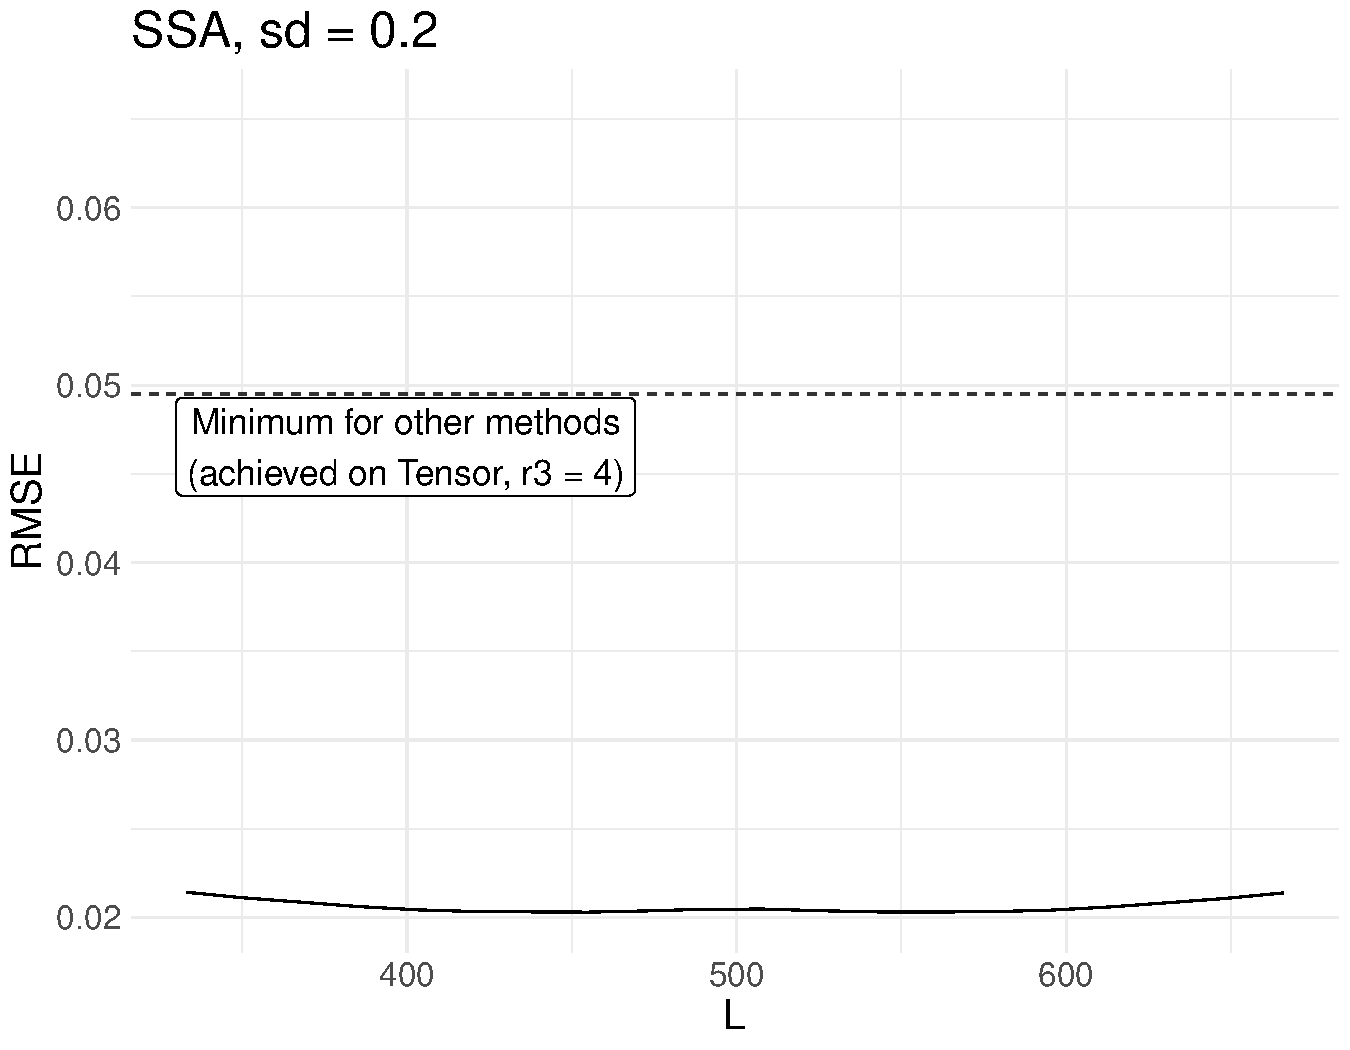
\includegraphics[width=\textwidth]{htlsd_byL_real_rec_rmse_ssa_2.pdf}
%     \end{minipage}
%     \begin{minipage}{0.48\textwidth}
%       \centering
%       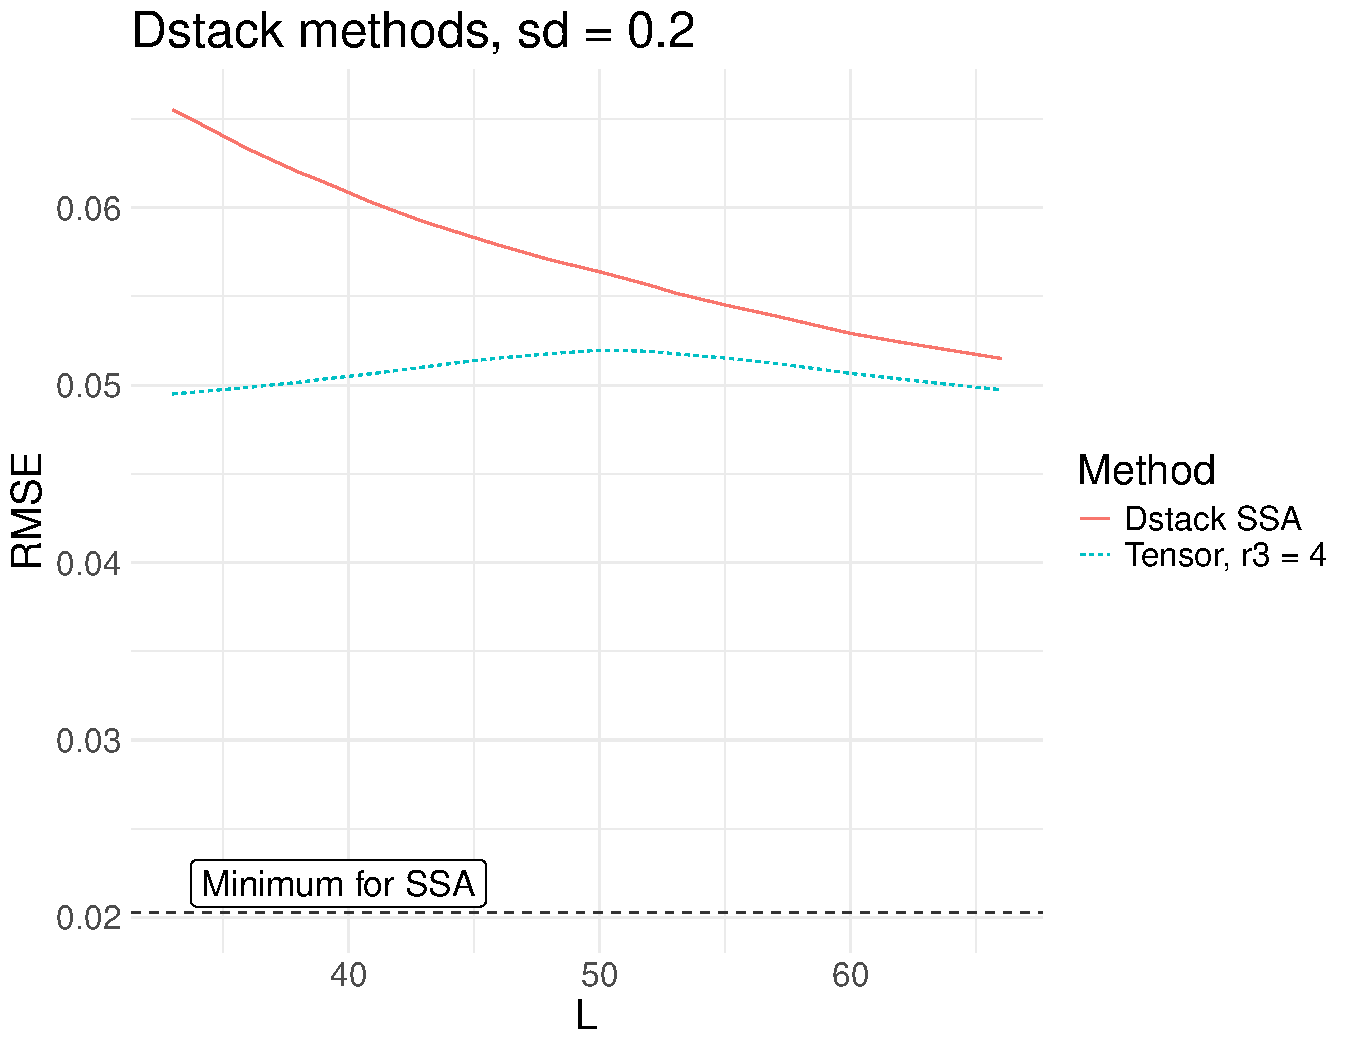
\includegraphics[width=\textwidth]{htlsd_byL_real_rec_rmse_dstack_2.pdf}
%     \end{minipage}
%     \caption{RMSE of signal estimate by default SSA
%     (left) and Dstack variant (right).}
%   \end{figure}
% \end{frame}

% \begin{frame}{Multi-Channel Case, Parameters Estimation}
%   \vspace*{-0.3cm}
%   \[
%     x_{n}^{(m)} = a_1^{(m)}
%     e^{2 \pi \mathrm{i} \omega_1 n} +
%     a_2^{(m)}
%     e^{2 \pi \mathrm{i} \omega_2 n} + \zeta_n^{(m)},
%   \]
%   $\zeta_n^{(m)}$ --- Complex white gaussian noise,
%   $\mathrm{D}\left(\zeta_n^{(m)}\right) = 0.2^2$, $\omega_1 = 0.2,\,
%   \omega_2 = 0.22$
%   \begin{figure}[!ht]
%     \centering
%     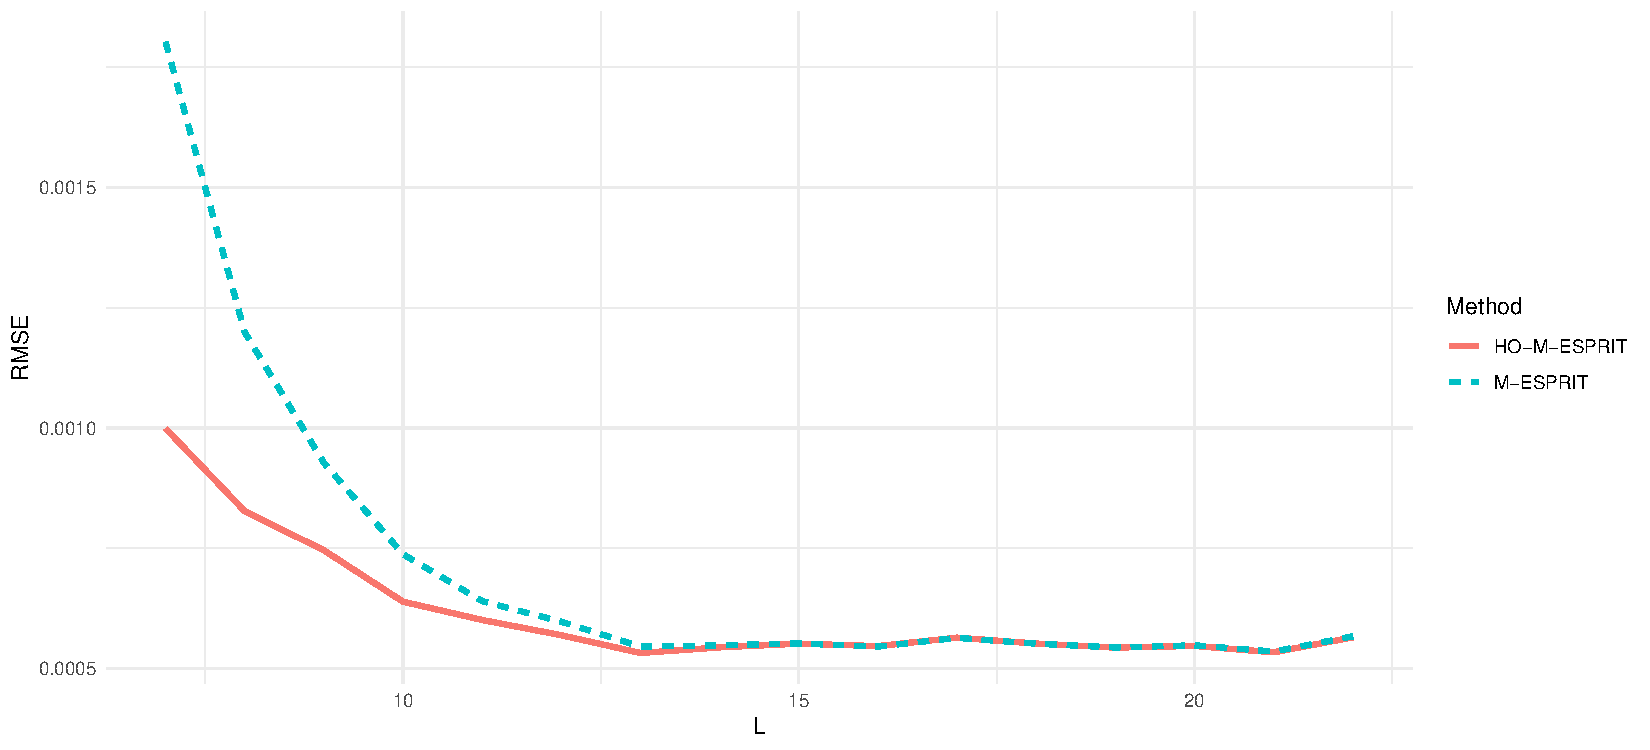
\includegraphics[width=0.87\textwidth]{img/freq1_L_no_rates.pdf}
%     \caption{RMSE of estimates for $\omega_1$ vs window length L.}
%   \end{figure}
% \end{frame}

% \begin{frame}{Multi-Channel Case, Signal Extraction}
%   \vspace*{-0.3cm}
%   \[
%     x_{n}^{(m)} = a_1^{(m)}
%     e^{2 \pi \mathrm{i} \omega_1 n} +
%     a_2^{(m)}
%     e^{2 \pi \mathrm{i} \omega_2 n} + \zeta_n^{(m)},
%   \]
%   $\zeta_n^{(m)}$ --- Complex white gaussian noise,
%   $\mathrm{D}\left(\zeta_n^{(m)}\right) = 0.2^2$, $\omega_1 = 0.2,\,
%   \omega_2 = 0.22$
%   \begin{figure}[!ht]
%     \centering
%     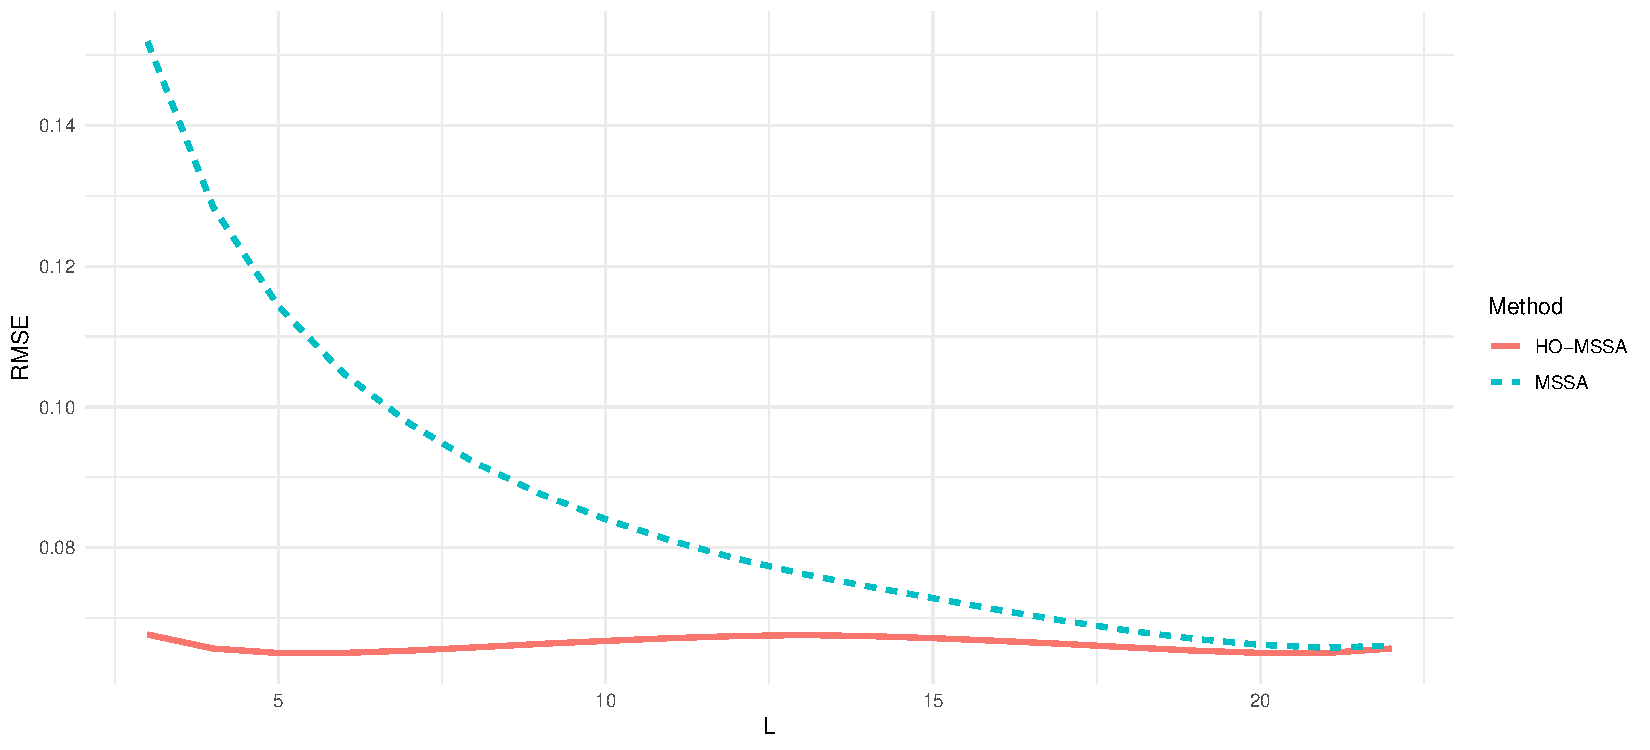
\includegraphics[width=0.87\textwidth]{img/rec_L_rmse_no_rates.pdf}
%     \caption{RMSE of signal estimation vs window length L.}
%   \end{figure}
% \end{frame}

\begin{frame}{Conclusions}
  \begin{itemize}
    \item Using High-Order SVD tensor decompositions instead of
      matrix SVD appears to be a more natural extension of the tensor
      that serves signal ranks. However, even in this case,
      truncation is not optimal for approximation, and ranks in
      different directions may differ.
      \smallskip
    \item HO-SSA is a natural extension of SSA, as are HO-M-SSA
      (signal extraction) and HO-ESPRIT and HO-M-ESPRIT (frequency estimation).
      \smallskip
    \item For optimal parameters, the accuracy of the tensor and
      matrix SSA/ESPRIT versions is comparable. The advantage of
      tensor-based methods is that they are generally less dependent
      on parameter choice (the worst and best parameter sets provide
      errors of the same order). However, the drawback is the
      complexity of tensor decompositions.
      \smallskip
    \item The HO-extension has fewer advantages for extracting
      one-dimensional signals. Therefore, this usage is not recommended.
      \smallskip
    \item Tensor methods using Dstack mapping can be useful for
      estimating parameters in the presence of strong noise.
  \end{itemize}
  %
  %  \vspace{0.3cm}

  %  \bluetext{For future:}
  %  \begin{itemize}
  %    \item Considering non-stationary signals
  %    \item Trying other tensor decompositions (CPD, T-SVD)
  %    \item Investigation of tensor modifications for other
  % SSA-based methods such that ...  (forecasting?)
  %    \item \dots
  %  \end{itemize}
\end{frame}

\begin{frame}[noframenumbering]{Algorithms Complexities}
  $\calX \in \bbC^{I\times L \times K}$, $\bfX \in \bbC^{\hat{L}
  \times \hat{K}}$, $I < L < K$, $\hat{L} < \hat{K}$,\\
  $I + L + K = N + 2$, $\hat{L} + \hat{K} = N + 1$
  \medskip
  \begin{itemize}
    \item \bluetext{SVD}$(\bfX)$:\\ $O(\hat{L}^2 \hat{K})$,\\ or
      $O(r\hat{L}\hat{K})$ if only
      need $r$-rank approximation,\\ or $O(r N \log (N))$ if $\bfX$ is Hankel
      \medskip
    \item \bluetext{HOSVD}$(\calX)$:\\ $O(ILKN)$,\\ or
      $O(ILK(r_1 + r_2 + r_3))$ if only need $(r_1, r_2, r_3)$-rank
      approximation,\\ or $O((r_1 + r_2 + r_3)I(L + K)\log(L + K))$ if
      $\calX$ is Hankel
      % \medskip
      % \item \bluetext{HOOI-SSA:}
      %   \[
      %     O(r_1 r_2 r_3 (I + L + J)),
      %   \]
      %   with linear convergence. For precision level of $\varepsilon$:
      %   \[
      %     O\left(ILJ(r_1 + r_2 + r_3) + \frac{1}{\varepsilon}r_1 r_2
      %     r_3 (I + L + J)\right)
      %   \]
  \end{itemize}
\end{frame}

\end{document}